\chapter{Elementary Differential Geometry}
\section{Fundamental conception on differential manifolds}
\begin{newdef}[Manifold]
\href{https://en.wikipedia.org/wiki/Manifold}{\textbf{Manifold}} 
Formally, a topological manifold is a second countable Hausdorff space that is locally homeomorphic to Euclidean space.\\
\href{https://en.wikipedia.org/wiki/Differentiable_manifold}{\textbf{Differentiable manifold}} 
In formal terms, a differentiable manifold is a topological manifold with a globally defined differential structure. \\
\href{https://en.wikipedia.org/wiki/Tangent_space}{\textbf{Tangent space}} 
In mathematics, the tangent space of a manifold facilitates the generalization of vectors from affine spaces to general manifolds, since in the latter case one cannot simply subtract two points to obtain a vector pointing from one to the other.\\
\href{https://en.wikipedia.org/wiki/Cotangent_space}{\textbf{Cotangent space}} 
Typically, the cotangent space is defined as the dual space of the tangent space at $x$.\\
\end{newdef}

\begin{newdef}[Submanifold]
\href{https://en.wikipedia.org/wiki/Submanifold}{\textbf{Submanifold}}\\
\textbf{Immersed submanifolds} An immersed submanifold of a manifold $M$ is the image $S$ of an immersion map $f:N \to M$; in general this image will not be a submanifold as a subset, and an immersion map need not even be injective (one-to-one) – it can have self-intersections.\\
\textbf{Injective immersion submanifolds} More narrowly, one can require that the map $f:N \to M$ be an inclusion (one-to-one), in which we call it an injective immersion, and define an immersed submanifold to be the image subset S together with a topology and differential structure such that S is a manifold and the inclusion f is a diffeomorphism: this is just the topology on N, which in general will not agree with the subset topology: in general the subset S is not a submanifold of M, in the subset topology.\\
\textbf{Open submanifolds}\\
\textbf{Closed submanifolds}\\
\end{newdef}

\begin{newdef}[Embedded Submanifold]
An embedded submanifold (also called a regular submanifold), is an immersed submanifold for which the inclusion map is a topological embedding. That is, the submanifold topology on $S$ is the same as the subspace topology. Given any embedding $f:N \to M$ of a manifold $N$ in $M$ the image $f(N)$ naturally has the structure of an embedded submanifold. That is, embedded submanifolds are precisely the images of embeddings.
\end{newdef}

\begin{newprop}[]
If an n dimensional injective immersed submanifold $N$ of a $m$ dimensional manifold $M$ is a closed submanifold of an open submanifold of $M$, then for every point $p \in f(N)$ there exists a chart ($U \subset M$,$\phi:U \to R_n $) containing $p$ such that $\phi(f(N) \cap U)$ is the intersection of a $n$-dimensional plane with $\phi(U)$.\\
Closed submanifolds of an open submanifold are equal to embedded submanifolds.
\end{newprop}

\section{Multi linear algebra}
\begin{newdef}[Tensor]
\textbf{Vector space}\\
\href{https://en.wikipedia.org/wiki/Dual_space}{\textbf{Dual space}}\\
In mathematics, any vector space $V$ has a corresponding dual vector space (or just dual space for short) consisting of all linear functionals on $V$ together with a naturally induced linear structure.\\
\textbf{Tensor product}
\[V \otimes W = \mbox{ Span}\{ v \otimes w \} = \mathcal{L}(V^*,W^*;F)\]
\[V^* \otimes W^* = \mbox{ Span}\{ v^* \otimes w^* \} = \mathcal{L}(V,W;F)\]
\[\mathcal{L}(V,W;Z)=\mathcal{L}(V \otimes W;Z)\]
\[(\phi \otimes \psi)\otimes \xi = \phi \otimes (\psi \otimes \xi)\]
\textbf{Tensor}
\[V_s^r = V \otimes \cdots \otimes V \otimes V^* \otimes \cdots \otimes V^*\]
\[x=x^{i_1 \cdots i_r}_{\phantom{i_1 \cdots i_r} k_1 \cdots k_s} e_{i_1} \otimes \cdots \otimes e_{i_r} \otimes e^{*k_1} \otimes \cdots \otimes e^{*k_s}\]
\[(x \otimes y)^{i_1 \cdots i_{r_1+r_2}}_{\phantom{i_1 \cdots i_{r_1+r_2}} k_1 \cdots k_{s_1+s_2}} = 
x^{i_1 \cdots i_{r_1}}_{\phantom{i_1 \cdots i_{r_1}}k_1 \cdots k_{s_1}} \cdot y^{i_{r_1+1} \cdots i_{r_1+r_2}}_{\phantom{i_{r_1+1} \cdots i_{r_1+r_2}}k_{s_1+1} \cdots k_{s_1+s_2}}\]
\end{newdef}

\begin{newdef}[Symmtric and antisymmetric tensor]
\textbf{Permutation}($\sigma \in \mathcal{P}(r)$)
\[\sigma x(v^{*1},\cdots,v^{*r})=x(v^{*\sigma(1)},\cdots,v^{*\sigma(r)})\]
\textbf{Symmetric contra-variant tensor}
\[\sigma x =x\]
\textbf{Antisymmetric contra-variant tensor}
\[\sigma x =\mbox{ sgn }\sigma \cdot x\]
\textbf{Symmetrization operator}
\[S_r(x) = \frac{1}{r!} \sum_{\sigma \in \mathcal{P}(x)} \sigma x\]
\textbf{Antisymmetrization operator}
\[A_r(x) = \frac{1}{r!} \sum_{\sigma \in \mathcal{P}(x)} \mbox{ sgn }\cdot \sigma x\]
\end{newdef}

\begin{newdef}[Exterior vector space]
\textbf{Exterior vector space}
\[\Lambda^r(V) = A_r(T^r(V))\]
\[\Lambda^0(V)=F \ \ \ \Lambda^1(V)=V\]
\textbf{Wedge product}
\[\xi \wedge \eta \equiv \frac{(k+l)!}{k!l!}A_{k+l}(\xi \otimes \eta)\]
\textbf{Pull-back mapping}
$f:V \to W$ is a linear mapping, we define $f^*:\Lambda^r(W^*) \to \Lambda^r(V^*)$ as
\[f^* \phi(v_1,\cdots,v_r) = \phi(f(v_1),\cdots,f(v_r)).\]
\end{newdef}

\begin{newprop}[Properties of Wedge product]
\[(\xi_1+\xi_2) \wedge \eta = \xi_1 \wedge \eta + \xi_2 \wedge \eta\]
\[\xi \wedge (\eta_1+\eta_2) = \xi \wedge \eta_1 + \xi \wedge \eta_2\]
\[\xi \wedge \eta = (-1)^{kl} \eta \wedge \xi\]
\[(\xi \wedge \eta) \wedge \zeta = \xi \wedge (\eta \wedge \zeta) = \frac{(k+l+h)!}{k!l!h!}A_{k+l+h}(\xi \otimes \eta \otimes \zeta)\]
\[f^*(\phi \wedge \psi) = f^*\phi \wedge f^*\psi\]
\end{newprop}

\begin{newprop}[Properties of exterior space]
\[e_{i_1} \wedge \cdots \wedge e_{i_r}(v^{*1},\cdots,v^{*r}) = \det \langle e_{i_{\alpha}},v^{*\beta} \rangle\]
\[e_{i_1} \wedge \cdots \wedge e_{i_r}(e^{*j_1},\cdots,e^{*j_r}) = \det \langle e_{i_{\alpha}},e^{*j_{\beta}} \rangle = \delta^{j_1 \cdots j_r}_{i_1 \cdots i_r}\]
\[\Lambda^r(V) = \mbox{ Span }\{e_{i_1} \wedge \cdots \wedge e_{i_r},1\leq i_1 < \cdots < i_r \leq n  \}\]
\[(\Lambda^r(V))^* = \Lambda^r(V^*)\]
\end{newprop}

\section{Vector Bundle}
\begin{newdef}[Fiber bundle]
\href{https://en.wikipedia.org/wiki/Fiber_bundle}{\textbf{Fiber bundle}} In mathematics, and particularly topology, a fiber bundle is a space that is locally a product space, but globally may have a different topological structure. Specifically, the similarity between a space E and a product space B × F is defined using a continuous surjective map $\pi :E \to B$ that in small regions of $E$ behaves just like a projection from corresponding regions of $B \times F$ to $B$. The map $\pi$, called the projection or submersion of the bundle, is regarded as part of the structure of the bundle. The space $E$ is known as the total space of the fiber bundle, $B$ as the base space, and $F$ the fiber.\\
\href{https://en.wikipedia.org/wiki/Vector_bundle}{\textbf{Vector Bundle}} 
In mathematics, a vector bundle is a topological construction that makes precise the idea of a family of vector spaces parameterized by another space $X$ (for example $X$ could be a topological space, a manifold, or an algebraic variety): to every point $x$ of the space $X$ we associate (or "attach") a vector space $V(x)$ in such a way that these vector spaces fit together to form another space of the same kind as $X$ (e.g. a topological space, manifold, or algebraic variety), which is then called a vector bundle over $X$.\\
\href{https://en.wikipedia.org/wiki/Tangent_bundle}{\textbf{Tangent bundle}} 
In differential geometry, the tangent bundle of a differentiable manifold $M$ is a manifold $TM$, which assembles all the tangent vectors in $M$. As a set, it is given by the disjoint union of the tangent spaces of $M$. That is,
\[
TM = \bigsqcup_{x \in M}T_xM = \bigcup_{x \in M} \{x\} \times T_xM = \bigcup_{x \in M}\{(x,y)| y \in T_xM \}
\]
where $T_xM$ denotes the tangent space to $M$ at the point $x$. So, an element of $TM$ can be thought of as a pair $(x,v)$ , where $x$ is a point in $M$ and $v$ is a tangent vector to $M$ at $x$. There is a natural projection $\pi : TM \to M$ defined by $\pi(x,v) = x$. This projection maps each tangent space $T_xM$ to the single point $x$. A section of $TM$ is a vector field on $M$, and the dual bundle to $TM$ is the cotangent bundle, which is the disjoint union of the cotangent spaces of $M$.\\
\textbf{Cotangent bundle} $T^*M = \bigcup_{x \in M} T^*_{\phantom{*}x}M$\\
\textbf{Tensor bundle} $T^r_sM = \bigcup_{x \in M} T^{r\phantom{x}}_{sx}M$\\
\end{newdef}


\section{Tangent vector field}
\begin{newthem}
Let $M$ be a smooth manifold, and let $Y:M \to TM$ be a vector field. If $(U, [x_i])$ is an arbitrary smooth coordinate chart on $M$, then $Y$ is smooth on $U$ if and only if its component functions with respect to this chart are smooth.
\end{newthem}

\begin{newthem}
Let $M$ be a $m$ dimensional smooth manifold and $v$ a smooth tangent vector field on $M$. $v:C^{\infty}(M) \to C^{\infty}$ satisfy that\\
(1) $\forall f,g \in C^{\infty}(M),v(f+g)=v(f)+v(g)$;\\
(2) $\forall f \in C^{\infty}(M),\alpha \in \bm{R},v(\alpha f)=\alpha \cdot v(f)$;\\
(3) $\forall f,g \in C^{\infty}(M),v(f\cdot g) = f \cdot v(g) + g \cdot v(f)$.\\
If $\alpha:C^{\infty}(M) \to C^{\infty}(M)$ satisfy the three conditions above, there exists a unique smooth vector field $v$ on $M$ that $\forall f \in C^{\infty}(M),v(f)=\alpha(f)$.
\end{newthem}

\begin{newthem}
$\forall X,Y \in \mathcal{H}(M),[X,Y]=X \circ Y -Y \circ X \in \mathcal{H}(M)$.
\end{newthem}

\begin{newprop}
(1) $[aX+bY,Z]=a[X,Z]+b[Y,Z]$;$[Z,aX+bY]=a[Z,X]+b[Z,Y]$;\\
(2) $[X,Y]=-[Y,X]$;\\
(3) $[X,[Y,Z]] + [Y,[Z,X]] +[Z,[X,Y]]=0$;\\
(4) $[X,Y]|_{U} = [X|_{U},Y|_{U}] = (X_i \frac{\partial Y^j}{\partial u^i} - Y^i \frac{\partial X^j}{\partial u^i}) \frac{\partial}{\partial u^j}$;\\
(5) $f_{*}[X,Y] = [f_{*}X,f_{*}Y]$;
\end{newprop}

\begin{newdef}[One parameter differentiable transformation group]
Let $M$ be a smooth manifold and $\phi:\bm{R} \times M \to M$ a smooth mapping, and $\forall (t,p) \in \bm{R} \times M$,denote $\phi_{t}(p) = \phi(t,p)$. If $\phi$ satisfy that\\
(1) $\phi_0 = \mathrm{id}:M \to M$;\\
(2) $\forall s,t \in \bm{R}, \phi_s \circ \phi_t = \phi_{s+t}$;\\
then $\phi$ is called a one parameter differentiable transformation group acting on $M$.\\
Trajectory of $\phi$ through $p$ on $M$:$\gamma_p(t) = \phi(t,p)$.\\
Vector field induced by $\phi$: $X_p(f) = \langle \gamma_p , f \rangle$.
\end{newdef}

\begin{newprop}
(1) $\gamma_q(t) = \phi(t,\phi(s,p)) = \phi(t+s,p) = \gamma_p(t+s)$;\\
(2) $(\phi_s)_{*}X_p = X_{\phi_s(p)}$;\\
(3) $\psi_{*} X_p = \tilde{X}_{\psi(p)}$ if $X$ is induced by $\phi$ and $\tilde{X}$ is induced by $\psi \circ \phi \circ \psi^{-1} $. $\psi$ is a smooth  homeomorphism.\\
(4) $[X,Y] = \lim_{t \to 0} \frac{Y_p-(\phi_t)_* Y_{\phi_{-t}(p)}}{t} = \lim_{t \to 0} \frac{(\phi_{-t})_*Y_{\phi_t(p)}- Y}{t}$ if $X$ is induced by $\phi$.
\end{newprop}

\begin{newdef}[Lie derivative]
\[\mathcal{L}_{X}Y \equiv \lim_{t \to 0} \frac{(\phi_{-t})_*Y_{\phi_t(p)}- Y}{t} =[X,Y]\]
\[\mathcal{L}_{X}f \equiv X(f)\]
\end{newdef}

\begin{newprop}
\[\mathcal{L}_{X}(Y + \lambda Z) = \mathcal{L}_{X}Y + \lambda\mathcal{L}_{X}Z\]
\[\mathcal{L}_{X}(f \cdot Y) = \mathcal{L}_{X}(f) \cdot Y + f\mathcal{L}_{X}Y\]
\[\mathcal{L}_{X}([Y,Z]) = [\mathcal{L}_{X}Y,Z]+ [Y,\mathcal{L}_{X}Z]\]
\end{newprop}

\begin{newthem}
Let $M$ be a n-dimensional smooth manifold and $X \in \mathcal{H}(M)$. If $p \in M$ and $X_p \neq 0$, $\exists (V,x^i)$ and $p \in V$ that $X|_V = \frac{\partial}{\partial y^1 }$
\end{newthem}

\begin{newdef}[Distribution]
\href{https://en.wikipedia.org/wiki/Distribution_(differential_geometry)}{\textbf{Distribution}} Let $M$ be a $C^{\infty }$  manifold of dimension $m$ , and let $n \leq m$ . Suppose that for each $x\in M$ , we assign an $n$-dimensional subspace $\Delta _{x}\subset T_{x}(M)$ of the tangent space in such a way that for a neighbourhood $N_{x}\subset M$ of $x$ there exist $n$ linearly independent smooth vector fields $X_{1},\ldots ,X_{n}$ such that for any point $y\in N_{x}$, $X_{1}(y),\ldots ,X_{n}(y)$ span $\Delta _{y}$. We let $\Delta$  refer to the collection of all the $\Delta_{x}$ for all $ x\in M$ and we then call $\Delta$ a distribution of dimension $n$ on $M$ , or sometimes a $C^{\infty }$ $n$-plane distribution on $M$. The set of smooth vector fields $\{X_{1},\ldots ,X_{n}\}$ is called a local basis of $\Delta$.
\end{newdef}

\begin{newdef}[Involutive distributions]
We say that a distribution $\Delta$ on $M$ is involutive if for every point $x \in M$ there exists a local basis $\{X_{1},\ldots ,X_{n}\}$ of the distribution in a neighbourhood of $x$ such that for all $1\leq i,j\leq n$ , $[X_{i},X_{j}]$  is in the span of $\{X_{1},\ldots ,X_{n}\}$.That is, if $[X_{i},X_{j}]$ is a linear combination of $\{X_{1},\ldots ,X_{n}\}$. Normally this is written as $ [\Delta ,\Delta ]\subset \Delta $.\\
Involutive distributions are the tangent spaces to foliations. Involutive distributions are important in that they satisfy the conditions of the Frobenius theorem, and thus lead to integrable systems.
A related idea occurs in Hamiltonian mechanics: two functions f and g on a symplectic manifold are said to be in mutual involution if their Poisson bracket vanishes.
\end{newdef}

\begin{newthem}[Frobenius Theorem]
 If distribution $\Delta$ on $M$ is involutive, then $\forall p \in M$, $\exists (V,x^i)$ and $p \in V$ that $\Delta|_{V} = \mathrm{Span} \{ \frac{\partial}{\partial y^1} , \cdots, \frac{\partial}{\partial y^h}\}$.
\end{newthem}

\begin{newdef}[Integrable manifold]
Let $L^{h}$ be a smooth distribution on $M$. If $\phi:N \to M$ is an injective immersion manifold, and $\forall p \in N$, $\phi_{*}(T_pN) \subset L^h(\phi(p))$, then $(\phi,N)$ is called an integrable manifold of $L^h$.\\
If $\forall q \in M$, there is an integrable manifold of $L^h$ through it, we say that $L^h$ is completely integrable.
\end{newdef}
\begin{newthem}
Let
\[\tau: \underbrace{A^1(M) \times \cdots \times A^1(M)}_p \times \underbrace{\mathcal{H}(M) \times \cdots \times \mathcal{H}(M)}_q \to c^{\infty}(M)\] 
be a $p+q$ multi-linear mapping, if $\forall 1 \leq a \leq p,1 \leq b \leq q$ and $\mu \in C^{\infty}(M)$,
\begin{eqnarray}
&&\tau(\alpha^1,\cdots,\mu \alpha^{a},\cdots,\alpha^p,v_1,\cdots,v_q)\nonumber \\
&=&\tau(\alpha^1,\cdots,\alpha^p,v_1,\cdots,\mu v_{b},\cdots,v_q)\nonumber \\
&=&\mu \cdot \tau(\alpha^1,\cdots,\alpha^p,v_1,\cdots,v_q)\nonumber
\end{eqnarray}
then the mapping $\tau$ define a $(p,q)$ tensor for all $x \in M$ smoothly.
\end{newthem}

\begin{newdef}[Lie derivatives]
Let $X$ be a smooth tangent vector field on $M$ and $\phi_t$ the one parameter differentiable transformation group inducing it. Denote the trajectory of $\phi_t$ through $x$ by $\gamma_x(t)$. So we have linear isomorphism
\[(\phi_t^{-1})_{*} = (\phi_{-t})_{*} : T_{\gamma_x(t)}M \to T_xM\]
\[(\phi_t)^* : T_{\gamma_x(t)}^* \to T_xM\]
So we can induce the linear isomorphism
\[\Phi_t: T^p_q(\gamma_x(t)) \to T^p_q(x)\]
If $S$ and $T$ are smooth tensor fields on $M$,\\
(1) for all $t$ which is small enough, $\Phi_tS$ is a smooth tensor field on $M$ which has the same type as $S$ ,and $\lim_{t \to 0} \Phi_t(S(\gamma_p(t))) = S(p),\forall p \in M$.\\
(2)$\Phi_t(S \otimes T) = \Phi_tS \otimes \Phi_tT$.\\
(3)$\Phi_t(C^a_b(S)) = C^a_b(\Phi_t(S))$, $C^a_b$ is a tag for contraction.\\
So,we can define the Lie derivative for smooth tensor field $\tau$ on $M$ as
\[\mathcal{L}_{X}(\tau) = \lim_{t \to 0}\frac{\Phi_t(\tau)-\tau}{t}\]
\end{newdef}

\begin{newprop}
\[\mathcal{L}_X(\tau_1+\lambda \tau_2) = \mathcal{L}_X \tau_1 + \lambda \mathcal{L}_X \tau_2\]
\[\mathcal{L}_X(\tau_1 \otimes \tau_2) = \mathcal{L}_X\tau_1 \otimes \tau_2 + \tau_1 \otimes \mathcal{L}_X \tau_2\]
\[C^r_s(\mathcal{L}_X \tau) = \mathcal{L}_X(C^r_s(\tau))\]
\[(\mathcal{L}_X \omega)(Y) = X(\omega(Y)) - \omega([X,Y])\]
\[\mathcal{L}_{[X,Y]} = \mathcal{L}_X \circ \mathcal{L}_Y - \mathcal{L}_Y \circ \mathcal{L}_X \]
\[\mathcal{L}_{X+Y} = \mathcal{L}_{X} + \mathcal{L}_{Y}\]
\end{newprop}

\begin{newprop}
\[((\mathcal{L}_X \tau)|_U)^{\mu_1,\cdots,\mu_p}_{v_1,\cdots,v_q} = X^{\alpha} \partial_{\alpha} \tau^{\mu_1,\cdots,\mu_p}_{v_1,\cdots,v_q} - \sum_{i=1}^{p} \tau^{\mu_1,\cdots,\alpha,\cdots,\mu_p}_{v_1,\cdots,v_q} \partial_{\alpha} X^{\mu_i} + \sum_{j=1}^{q}\tau^{\mu_1,\cdots,\mu_p}_{v_1,\cdots,\alpha,\cdots,v_q} \partial_{v_j}X^{\alpha}\]
\end{newprop}

\section{Exterior differential}
\begin{newdef}[Exterior form space]
$A(M) = \sum_{r=0}^{m} A^{r}(M)$\\
For $\tau \in A^r(M)$,
\[\tau|_{U} = \frac{1}{r!} \tau_{i_1\cdots i_r} dx^{i_1} \wedge \cdots \wedge dx^{i_r} = \tau_{|i_1\cdots i_r|} dx^{i_1} \wedge \cdots \wedge dx^{i_r}\] 
\[ \tau_{i_1\cdots i_r} = \tau(\frac{\partial}{\partial x^{i_1}},\cdots,\frac{\partial}{\partial x^{i_r}}) \]
\begin{eqnarray}
\tau(v_1,\cdots,v_r)|_{U} &=& \tau_{|i_1\cdots i_r|}dx^{i_1} \wedge \cdots \wedge dx^{i_r} (v_1,\cdots,v_r) \nonumber \\
&=& \tau_{|i_1\cdots i_r|} \left| \begin{matrix} v_1^{i_1}& \cdots & v_r^{i_1}\\ \vdots & & \vdots \\ v_1^{i_r} & \cdots & v_r^{i_r} \end{matrix} \right| \nonumber
\end{eqnarray}
It is a $r$ multi-linear mapping, and for every variable, it is $C^{\infty}(M)$ linear.
\end{newdef}

\begin{newprop}[Pullback mapping]
$f:M \to N \Rightarrow f_{*}:T_{p}M \to T_{f(p)}N \Rightarrow f^{*}:\wedge^{r}(T_{f(p)}^{*}N) \to \wedge^{r}(T_p^*M) $\\
\[f^* \phi(v_1,\cdots,v_r) = \phi(f_*v_1,\cdots,f_*v_r)\]
\[f^*\phi|_U = \frac{1}{r!}(\phi_{\alpha_1\cdots\alpha_r} \circ f) \cdot \frac{\partial f^{\alpha_1}}{\partial x^{i_1}} \cdots \frac{\partial f^{\alpha_r}}{\partial x^{i_r}} dx^{i_1} \wedge \cdots \wedge dx^{i_r}\]
\[f^*(\phi \wedge \psi) = f^*\phi \wedge f^* \psi\]
\end{newprop}

\begin{newdef}[Exterior differential]
Let $M$ be a m-dimensional smooth manifold. Then $\exists$ a unique mapping $d:A(M) \to A(M)$ satisfy that\\
(1) $d(A^r(M)) \subset A^{r+1}(M)$\\
(2) $\forall \omega_1,\omega_2 \in A(M),d(\omega_1+\omega_2) = d\omega_1 +d\omega_2$\\
(3) if $\omega_1 \in A^r(M)$,then $d(\omega_1 \wedge \omega_2)=d\omega_1 \wedge \omega_2 +(-1)^r \omega_1 \wedge d\omega_2$\\
(4) $f \in A^0(M)$,$df$ is just the differential of $f$\\
(5) $\forall f \in A^0(M)$,$d(df)=0$\\
$d$ is called exterior differential.
\end{newdef}

\begin{newthem}
$\forall \omega \in A^1(M),X,Y \in \mathcal{H}(M)$,
\[d\omega(X,Y) = X \langle Y,\omega \rangle -Y \langle X,\omega \rangle -\langle [X,Y],\omega \rangle \] 
$\forall \omega \in A^r(M)$, $X_1,\cdots,X_{r+1} \in \mathcal{H}(M)$,
\begin{eqnarray}
d\omega(X_1,\cdots,X_{r+1}) &=& \sum_{i=1}^{r+1}(-1)^{i+1} X_{i}(\langle X_1 \wedge \cdots \wedge \hat{X_i} \wedge \cdots \wedge X_{r+1},\omega \rangle) \nonumber \\
&+& \sum_{1 \leq i < j \leq r+1}(-1)^{i+j} \langle [X_i,X_j] \wedge \cdots \wedge \hat{X_i} \wedge \cdots \wedge \hat{X_j} \wedge \cdots X_{r+1},\omega \rangle \nonumber
\end{eqnarray}
\end{newthem}

\begin{newthem}
\[f^{*}(d\omega) = d(f^* \omega)\]
\end{newthem}

\begin{newlemma}[Poincare Lemma]
\begin{enumerate}
\item $d^2=0$
\item Let $U=B_0(r)$ be a spherical neighbourhood with center origin $O$ and radius $r$ in $R^n$. $\forall \omega \in A^r(U)$ and $d\omega =0$, $\exists \tau \in A^{r-1}(U)$,satisfy that $\omega = d\tau$.
\end{enumerate}
\end{newlemma}

\begin{newdef}[Pfaff euqations]
Let $\omega^{\alpha}(1 \leq \alpha \leq r) \in A^1(U)$ and $U$ is an open set of $m$-dimensional smooth manifold $M$. Differential equation set $\omega^{\alpha} = 0$ is called Pfaff equations.
\end{newdef}

\begin{newdef}[Integral manifold of Pfaff equations]
If there is an injective immersion submanifold $\phi:N \to U$ satisfying that $\phi^{*} \omega^{\alpha} = 0$,$(\phi,N)$ is called an integral manifold of Pfaff eqation set.
\end{newdef}

\begin{newprop}[Partial differential equations and Pfaff equations]
There is a set of first order partial differential equations
\[\frac{\partial y^{\alpha}}{\partial x^i} = f^{\alpha}_{i}(x^1,\cdots,x^{m},y^1,\cdots,y^{n}) \ \ \ (1 \leq i \leq m,1 \leq \alpha \leq n)\]
$f^{\alpha}_{i}(x,y)$ is a smooth function on the open set $U \times V \subset R^m \times R^n$. The equations sets can be written as Pfaff equations on $U \times V$
\[\omega^{\alpha} \equiv dy^{\alpha} - f^{\alpha}_{i}(x,y)dx^i = 0\]
If the partial differential equations have solution
\[y^{\alpha} = g^{\alpha}(x^1,\ldots,x^m)\]
then the submanifold $\phi:U \to U \times V$,
\[\phi(x^1,\ldots,x^m) = (x^1,\ldots,x^m,g^1(x),\ldots,g^n(x))\]
is an integral manifold of the Pfaff equations , i.e. $\phi^* \omega^{\alpha} =0$
\end{newprop}

\begin{newprop}[Distribution and Pfaff equations]
Pfaff equations $\omega^{\alpha} = 0$ on open set $V \in M$ with rank $r$ is equivalent to a $h=m-r$ dimensional smooth distribution locally.
\[\Delta^h(p) = \{v \in T_pM:\omega^{\alpha}(v)=0,1 \le \alpha \le r \}\]
If $\phi:N \to V$ is an integral manifold of $\omega^{\alpha}$,$\forall X \in T_pN$,$\omega^{\alpha}(\phi_{*}X) = \phi^* \omega_{\alpha}(X) =0$. So $\phi_* X \in \Delta^h(p)$, and so $\phi:N \to V$ is an integral manifold of $\Delta^h$.
\end{newprop}

\begin{newdef}[Completely integrable]
Suppose $\omega^{\alpha}$ is a set of $r$ linearly independent 1 forms defined on an open set $U \subset M$. If $\forall p \in U$,  Paffa equations
\[\omega^{\alpha} = 0 \quad (1 \leq \alpha \leq r)\]
has an $h = \dim M -r$ dimensional integral manifold $\phi: N \to V$ such that $p \in V$, Paffa equations are called completely integrable.
\end{newdef}     

\begin{newdef}[Frobenius condition]
Frobenius condition for Pfaff equations $\omega^{\alpha} =0(1 \le \alpha \le r)$ is that
\[d\omega^{\alpha} \wedge \omega^1 \wedge \cdots \wedge \omega^r = 0\]
\end{newdef}

\begin{newthem}[Frobenius theorem]
Pfaff equations satisfying Frobenius condition is completely integrable.
\end{newthem}

\begin{newdef}[Orientation of manifold]
Let $\alpha:[0,1] \to M$ be a path on $M$. $\forall t \in [0,1]$, assign an orientation for $T_{\alpha(t)}M$, denoted by $\mu_t$. If for $t_0 \in [0,1]$, there is a local coordinate $(U;x_i)$ of $\alpha(t_0)$ and a neighbourhood $[t_0-\delta_1,t_0+\delta_2]$ of $t_0$ that
\[\alpha([t_0-\delta_1,t_0+\delta_2]) \subset U\] 
and
\[\left\{ \frac{\partial}{\partial x^1},\ldots,\frac{\partial}{\partial x^m}\right\}|_{\alpha(t)} \in \mu_t,\forall t \in [t_0-\delta_1,t_0+\delta_2],\] 
$\mu$ is called a continuous topological orientation of $\alpha$
\end{newdef}

\begin{newdef}[The propagation of orientation]
Let $p,q \in M$ and $\alpha:[0,1] \to M$ a path connecting $p,q$. Assign an orientation $\lambda$ of $T_pM$. If there is a continuous topological orientation of $\alpha$ $\mu$ satisfying that $\mu_0 = \lambda$, then orientation $\mu_1$ of $T_qM$ is called the propagation of orientation $\lambda$ along $\alpha$. The orientation of $\mu_1$ is unique.
\end{newdef}

\begin{newdef}[Orientable manifold]
 Let $M$ be a $m$ dimensional smooth manifold. If there is an atlases $(\mathcal{A_0} = \{(U_{\alpha},\phi_{\alpha})\})$, making that if $U_{\alpha} \cap U_{\beta} \neq \emptyset$,the Jacobian of
\[\phi_{\beta} \circ \phi_{\alpha}^{-1} : \phi_{\alpha}(U_{\alpha} \cap U_{\beta}) \to \phi_{\beta}(U_{\alpha} \cap U_{\beta})\]
is positive. Then $M$ is called orientable manifold.
\end{newdef}

\begin{newthem}
Let $M$ be a orientable connected manifold. $\forall p \in M$,assign an orientation $\lambda$ for $T_pM$, then for all point $q \in M$, the propagation of $\lambda$ along an arbitrary path define a unique orientation $\mu$ for $T_q M$.
\end{newthem}

\begin{newdef}[Manifold with boundary]
A topological manifold with boundary is a Hausdorff space in which every point has a neighbourhood homeomorphic to an open subset of Euclidean half-space (for a fixed $n$):
\[\mathbb {R} _{+}^{n}=\{(x_{1},\ldots ,x_{n})\in \mathbb {R} ^{n}:x_{n}\geq 0\}\]
\end{newdef}


\begin{newdef}[Boundary and interior]
Let M be a manifold with boundary. The interior of $M$, denoted $Int \ M$, is the set of points in $M$ which have neighbourhoods homeomorphic to an open subset of $\mathbb {R} ^{n}$. The boundary of $M$, denoted $\partial M$, is the complement of $Int \ M$ in $M$. The boundary points can be characterized as those points which land on the boundary hyperplane ($x^n=0$) of $ \mathbb {R} _{+}^{n}$ under some coordinate chart.\\
If $M$ is a manifold with boundary of dimension $n$, then $Int \ M$ is a manifold (without boundary) of dimension $n$ and $\partial M$ is a manifold (without boundary) of dimension $n-1$.
\end{newdef}

\begin{newthem}
Let $M$ be a smooth manifold with boundary and $\partial M \neq \emptyset$. The differential structure of $\partial M$ can be deduced from the $M$, making $\partial M$ a $m-1$ dimensional smooth manifold and the inclusion map $i:\partial M \to M$ is embedding map. If $M$ is orientable, then $\partial M$ is also orientable.
\end{newthem}

\begin{newdef}[Induced orientation] 
Let $M$ be an orientable $m$ dimensional smooth manifold with boundary and $\partial M \neq \emptyset$. $\mathcal{A}$ is the orientation of $M$. For local coordinates $(U;x^i) \in \mathcal{A}$, when 
\[\tilde{U} = U \cap \partial M = \{(x^1,\ldots,x^m) \in U:x^m=0 \} \neq \emptyset\]
assign a local coordinate system $((-1)^m \cdot x^1,x^2,\ldots,x^{m-1})$ on $\tilde{U}$. The orientation defined by this local coordinate system is called induced orientation of $\partial M$.
\end{newdef}

\begin{newdef}[Support set] 
Let $M$ be a $m$ dimensional orientable smooth manifold. $\omega \in A^r(M)$, the support set of $\omega$ can be defined as
\[Supp \ \omega = \overline {\{ p \in M :\omega(p) \neq 0\}}\]\\
All the $r$-form with compact support set is denoted as $A^r_0(M)$.
\end{newdef}

\begin{newdef}[Partition of unity]
Let $\Sigma$ be an open cover of $M$. Then there is a family of smooth function $g_{\alpha}$ on $M$ that
\begin{enumerate}
\item $\forall \alpha$,$0 \leq g_{\alpha} \leq 1$,$\mathrm{supp} \ g_{\alpha}$ is compact and there is an open set $W_i \in  \Sigma$ that $\mathrm{supp} \  g_{\alpha} \subset W_i$.
\item $\forall p \in M$, it has a neighbourhood $U$ which intersect finite $\mathrm{supp} \ g_{\alpha}$.
\item $\sum_{\alpha} g_{\alpha} = 1$
\end{enumerate}
\end{newdef}


\begin{newdef}[Integral of differential form with compact support]
\[\phi = (\sum_{\alpha} g_{\alpha})\cdot \phi = \sum_{\alpha} (g_{\alpha} \cdot \phi)\]
\[\int_{M} g_{\alpha} \cdot \phi = \int_{W_i} g_{\alpha} \cdot \phi = \int_{W_i} f(u^1,\cdots,u^m) du^1 \wedge \cdots \wedge du^m = \int_{W_i} f(u^1,\cdots,u^m) du^1 \cdots du^m\]
\[\int_{M} \phi = \sum_{\alpha} \int_{M} g_{\alpha} \cdot \phi\]
\end{newdef}

\begin{newthem}[Stokes Theorem] 
Let $M$ be an orientable $m$ dimensional smooth manifold with boundary and $\omega \in A_0^{m-1}(M)$,then
\[\int_{M} d\omega = \int_{\partial M} i^* \omega\]
Here, $\partial M$ has an orientation induced by $M$ and $i$ is  embedding mapping.
\end{newthem}

\section{Connection}
\begin{newdef}[Connection] 
Let $M$ be a smooth manifold and $E$ a $q$ dimensional real vector bundle on $M$. $\Gamma(E)$ is the set of all smooth sections of $E$ on $M$. The connection on $E$ is a mapping:
\[D:\Gamma(E) \to \Gamma(T^*(M) \otimes E)\]
it satisfies that
\begin{enumerate}
\item $\forall s_1 ,s_2 \in \Gamma(E)$,$D(s_1+s_2) = Ds_1+Ds_2$
\item $\forall s \in \Gamma(E)$ and $\alpha \in C^{\infty}(M)$, $D(\alpha s) = d\alpha \otimes s + \alpha Ds$
\end{enumerate}
If $X$ is a smooth tangent vector field on $M$, $s \in \Gamma(E)$,then
$D_{X}s = \langle X, Ds \rangle$, called absolute derivative of $s$ along $X$.
\end{newdef}

\vspace{50pt}

\begin{newprop}
Local representation of connection is: 
\[Ds_{\alpha} = \sum_{1 \leq i \leq m,1 \leq \beta \leq q} \Gamma^{\beta}_{\alpha i} du^i \otimes s_{\beta}\]
\[\omega^{\beta}_{\alpha} = \sum_{1 \leq i \leq m} \Gamma^{\beta}_{\alpha i} du^i\]
\[Ds_{\alpha} = \sum_{\beta=1}^{q} \omega^{\beta}_{\alpha} \otimes s_{\beta}\]
\[DS = \omega \otimes S\]
Transformation law of connection is:
\[S' = A \cdot S\] 
\begin{eqnarray}
DS' &=& dA \otimes S + A \cdot DS \nonumber \\
&=& (dA + A \cdot \omega) \otimes S \nonumber \\
&=& (dA \cdot A^{-1} + A \cdot \omega \cdot A^{-1}) \otimes S' \nonumber
\end{eqnarray}
\[\omega' = dA \cdot A^{-1} + A \cdot \omega \cdot A^{-1}\]
\end{newprop}

\begin{newthem}
For an arbitrary vector bundle, connection always exists.
\end{newthem}

\begin{newthem} 
Let $D$ be a connection of vector bundle $E$. $\forall p \in M$, there exists a local frame field $S$ on the neighbourhood of $p$ that $\omega(p) =0$.
\end{newthem}

\begin{newdef}[Curvature matrix]
\[\Omega \equiv d\omega - \omega \wedge \omega\]
\end{newdef}

\begin{newprop}[Transformation law of curvature matrix]
\[\Omega' = A \cdot \Omega \cdot A^{-1}\]
\end{newprop}

\begin{newdef}[Curvature operator]
\[s = \sum_{\alpha=1}^{q} \lambda^{\alpha} s_{\alpha|p}\]
\[R(X,Y)s = \sum_{\alpha,\beta=1}^{q} \lambda^{\alpha} \Omega^{\beta}_{\alpha}(X,Y)s_{\beta|p}\]
\[(R(X,Y)s)(p) = R(X_p,Y_p)s_p\]
\end{newdef}

\begin{newprop}
\[R(X,Y) = D_X D_Y - D_Y D_X -D_{[X,Y]}\]
\end{newprop}

\begin{newthem}[Bianchi equation]
\[d\Omega = \omega \wedge \Omega - \Omega \wedge \omega\]
\end{newthem}

\begin{newdef}[Induced connection]
\[d\langle s,s^* \rangle = \langle Ds,s^* \rangle + \langle s,Ds^* \rangle\]
\[\langle s_{\alpha},s^{*\beta} \rangle  = \delta^{\beta}_{\alpha}  \Rightarrow Ds^{*\beta} = -\sum_{\alpha=1}^{q} \omega^{\beta}_{\alpha} \otimes s^{*\alpha}\]
\[D(s_1 \oplus s_2) \equiv Ds_1 \oplus Ds_2\]
\[D(s_1 \otimes s_2) \equiv Ds_1 \otimes s_2 + s_1 \otimes Ds_2\]
\end{newdef}

\begin{newdef}[Affine connection]
\[D\frac{\partial}{\partial u^i} \equiv \omega^j_i \otimes \frac{\partial}{\partial u^j} \equiv \Gamma^{j}_{ik} du^k \otimes \frac{\partial}{\partial u^j}\]
\end{newdef}

\begin{newprop}
\[\Gamma'^{j}_{ik} = \Gamma^{q}_{pr} \frac{\partial w^j}{\partial u^q} \frac{\partial u^p}{\partial w^i} \frac{\partial u^r}{\partial w^k} + \frac{\partial^2 u^p}{\partial w^i \partial w^k} \frac{\partial w^j}{\partial u^p}\]
\[DX = (dX^i + x^j \omega^i_j)\otimes \frac{\partial}{\partial u^i} = (X^i_{,j} + X^k \Gamma^{i}_{kj}) du^j \otimes \frac{\partial}{\partial u^i} = X^i_{;j}du^j \otimes \frac{\partial}{\partial u^i} \]
\[D \alpha = (d\alpha_i - \alpha_j \omega^j_i)\otimes du^i = (\alpha_{i,j} -\alpha_k \Gamma^k_{ij})du^j \otimes du^i = \alpha_{i;j} du^j \otimes du^i \]
\end{newprop}

\begin{newdef}[Geodesic equation]
\[\frac{D(\frac{du^i(t)}{dt} \frac{\partial}{\partial u^i})}{dt} = 0 \]
\[\frac{d^2 u^i}{dt^2} + \Gamma^i_{jk} \frac{du^j}{dt} \frac{du^k}{dt} = 0\]
\end{newdef}

\begin{newdef}[Curvature tensor]
\[\Omega^j_i = \frac{1}{2}R^j_{ikl} du^k \wedge du^l \]
\[R \equiv R^{j}_{ikl} du^{i} \otimes \frac{\partial}{\partial u^j} \otimes du^{k} \otimes du^{l}\]
\end{newdef}

\begin{newprop}
\[R^j_{ikl} = \frac{\partial \Gamma^j_{il}}{\partial u^k} - \frac{\partial \Gamma^j_{ik}}{\partial u^l} + \Gamma^h_{il} \Gamma^j_{hk} - \Gamma^h_{ik} \Gamma^j_{hl}\]
\[R'^j_{ikl} = R^q_{prs} \frac{\partial w^j}{\partial u^q} \frac{\partial u^p}{\partial w^i} \frac{\partial u^r}{\partial w^k}\frac{\partial u^s}{\partial w^l}\]
\[R(X,\alpha_Y,Z,W)= \langle \alpha_Y,R(Z,W)X \rangle\]
\[R^{j}_{ikl} = \langle R(\frac{\partial}{\partial u^k} \frac{\partial}{\partial u^l})\frac{\partial}{\partial u^i},du^j \rangle\]
\end{newprop}


\begin{newdef}[Torsion tensor]
\[T^j_{ik} = \Gamma^j_{ki} - \Gamma^j_{ik}\]
\[T = T^j_{ik} \frac{\partial}{\partial u^j} \otimes du^i \otimes du^k\]
\end{newdef}

\begin{newprop}
\[T(X,Y) = T^k_{ij}X^i Y^j \frac{\partial}{\partial u^k}\]
\[T(X,Y) = D_X Y - D_Y X - [X,Y]\]
\end{newprop}

\begin{newthem}
Let $D$ be an affine connection without torsion on $M$. $\forall p \in M$, there is a local coordinate system that $\Gamma^j_{ik}(p)$ vanishes.
\end{newthem}

\begin{newthem}
Let $D$ be an affine connection without torsion on $M$. Then we have Bianchi equation
\[R^j_{ikl;h} + R^j_{ihk;l} + R^j_{ilh;k} = 0\]
\end{newthem}

\section{Riemann manifold}
\begin{newdef}[Riemann manifold] 
Let $M$ be a smooth manifold equipped with a smooth non-degenerate symmetric second order covariant tensor field $G$, then $M$ is called general Riemann manifold and $G$ is called the metric tensor of $M$.\\
If $G$ is positive definite, then $M$ is called Riemann manifold.
\end{newdef}

\vspace{15pt}

\begin{newthem}
There must be a Riemann metric on $m$ dimensional manifold $M$.
\end{newthem}

\vspace{15pt}

\begin{newdef}[Index lifting]
\[f:T_p(M) \to T^*_p(M) \quad \alpha_X(Y) \equiv G(X,Y)\]
\end{newdef}

\vspace{15pt}

\begin{newdef}[Adapted connection]
Let $(M,G)$ be a general Riemann manifold and $D$ a connection on $M$. If $DG=0$,then $D$ is called adapted connection on $M$.
\end{newdef}

\vspace{15pt}

\begin{newprop}[Christoffel-Levi-Civita connection] 
Let $M$ be a general Riemann manifold, then there is a unique adapted connection without torsion on $M$, called Christoffel-Levi-Civita connection. \\
As $\omega^{j}_{i} = \Gamma^{j}_{ik}du^k$, $dg_{ij} = g_{ik}\omega^{k}_{j} + g_{kj}\omega^{k}_{i}$.
If we denote that $\omega_{ij} = \omega_{i}^{j}g_{jk}$ and $\Gamma_{ijk} = \Gamma_{ik}^{l}g_{lj}$, we have $\omega_{ij}=\Gamma_{ijk}du^k$ and $dg_{ij} = \omega_{ji}+ \omega_{ij}$.
At last, we have
\[\Gamma^{k}_{ij} = \frac{1}{2} g^{kl}(\frac{\partial g_{il}}{\partial u^j} + \frac{\partial g_{jl}}{\partial u^i} - \frac{\partial g_{ij}}{\partial u^l})\]
\end{newprop}

\begin{newprop}[Curvature tensor]
If we denote that $\Omega_{ij} = \Omega_{i}^{k}g_{kj}$ and $R_{ijkl} = R^{h}_{ikl}g_{hj}$, we will have that
\[\Omega_{ij} + \Omega_{ji} = 0,\ \ \Omega_{ij} = d\omega_{ij} + \omega_{i}^{l} \wedge \omega_{jl},\ \ \Omega_{ij} = \frac{1}{2}R_{ijkl}du^k \wedge du^l\]
The properties of curvature tensor:
\[R_{ijkl} = -R_{jikl} = -R_{ijlk}\]
\[R_{ijkl}+R_{iklj}+R_{iljk}=0\]
\[R_{ijkl} = R_{klij}\]
\end{newprop}

\begin{newdef}[\href{https://en.wikipedia.org/wiki/Normal_coordinates}{\textbf{Normal coordinates}}]
In differential geometry, normal coordinates at a point $p$ in a differentiable manifold equipped with a symmetric affine connection are a local coordinate system in a neighbourhood of $p$ obtained by applying the exponential map to the tangent space at $p$. In a normal coordinate system, the Christoffel symbols of the connection vanish at the point $p$, thus often simplifying local calculations. In normal coordinates associated to the Levi-Civita connection of a Riemann manifold, one can additionally arrange that the metric tensor is the Kronecker delta at the point $p$, and that the first partial derivatives of the metric at $p$ vanish.\\
The properties of normal coordinates often simplify computations. In the following, assume that $U$ is a normal neighbourhood centred at $p$ in $M$ and ($x_i$) are normal coordinates on $U$.\\
Let $V$ be some vector from $T_pM$ with components $V^i$ in local coordinates, and $\gamma_V$ be the geodesic with starting point $p$ and velocity vector $V$, then $\gamma_V$ is represented in normal coordinates by $\gamma _{V}(t)=(tV^{1},...,tV^{n})$ as long as it is in $U$.\\
The coordinates of $p$ are $(0, \cdots, 0)$\\
In Riemann normal coordinates at p the components of the Riemann metric $g$ simplify to $\delta _{ij}$.\\
The Christoffel symbols vanish at $p$. In the Riemann case, so do the first partial derivatives of $g_{ij}$.
\end{newdef}

\begin{newthem}
Let $M$ be a differentiable manifold equipped with a symmetric affine connection. $\forall x_0 \in M$, there is a neighbourhood $W$ that for every point in $W$, there is a neighbourhood equipped with a normal coordinate system which contains $W$.
\end{newthem}

\begin{newthem}
Let $M$ be a Riemann manifold. $\forall O \in M$,there is a neighbourhood with normal coordinates $W$ that:\\
(1) For every point in $W$, there is a neighbourhood equipped with a normal coordinates which contains $W$.\\
(2) The geodesic connecting $O$ and $p \in W$ is the only shortest path connecting these two points in $W$.
\end{newthem}

\begin{newthem}
Let $U$ be the neighbourhood with normal coordinates of $O$. $\exists \epsilon >0, \forall \delta \in (0,\epsilon)$,the surface
\[\Sigma_{\delta} = {p \in U | \sum_{i=1}^{m}} (u^i(p))^2 = \delta^2\]
has following properties:\\
(1) $\forall p \in \Sigma_{\delta}$, there is a unique shortest geodesic connecting $p$ and $O$ in $U$.\\
(2) For all geodesics tangent to $\Sigma_{\delta}$, there is a neighbourhood of the cut point in which the geodesics lies outside of $\Sigma_{\delta}$
\end{newthem}

\begin{newthem}
Let $M$ be a Riemann manifold and $\forall p \in M$, there is a $\eta$-spherical neighbourhood $W$ that for arbitrary two points in $W$, there is a unique geodesic connecting these two points.
\end{newthem}

\begin{newdef}[Cross section curvature]
\[R(X,Y,Z,W) \equiv R_{ijkl}X^iY^jZ^kW^l\]
\[R(X,Y,Z,W) = (R(Z,W)X) \cdot Y\]
\[G(X,Y,Z,W) \equiv G(X,Z)G(Y,W) - G(X,W)G(Y,Z)\]
Let $E$ be a two dimensional subspace of $T_p(M)$ and $X,Y$ two linearly independent tangent vector of $E$,then
\[K(E) = -\frac{R(X,Y,X,Y)}{G(X,Y,X,Y)}\]
is a function of $E$, which is independent of the choice of $X,Y$,called cross section curvature.
\end{newdef}

\begin{newthem} 
Let $M$ be a Riemann space. The curvature tensor of $p \in M$ is uniquely determined by the cross section curvature of all the two dimensional subspace of $T_p(M)$.
\end{newthem}

\begin{newdef}[Constant curvature Riemann manifold]
Let $M$ be a Riemann manifold. If all of $K(E)$ on $p$ is constant, then $M$ is called isotropic on $p$. \\
If $M$ is isotropic every where and $K(p)$ is constant over $M$, then $M$ is called constant curvature Riemann manifold.
\end{newdef}

\begin{newthem}[F.Schur theorem] 
Let $M$ be a $m$-dimensional connected Riemann manifold that is isotropic every where. If $m \geq 3$, then $M$ is constant curvature Riemann manifold.
\end{newthem}

\chapter{A Geometrical Description of Newton Theory}
\section{Introduction}
\noindent
We choose Euclidean coordinates for our absolute space and an absolute time $t$, than the equation of motion can be written as
\[\frac{d^2 t}{d\lambda^2} = 0\]
\[\frac{d^2 x^i}{d\lambda^2} + \frac{\partial \Phi}{\partial x^i} (\frac{d\lambda}{dt})^2=0\]
It is convenient to define that $\Gamma^i_{00} = \frac{\partial \Phi}{\partial x^i}$,and all other $\Gamma^{\alpha}_{\beta \gamma}$ vanish.Then we can write the equation of motion as
\[\frac{d^2 x^{\alpha}}{d\lambda^2} + \Gamma^{\alpha}_{\beta \gamma} \frac{dx^{\beta}}{d \lambda} \frac{dx^{\gamma}}{d \lambda}=0\]
Next, we can get the Riemann tensor given the connection above\[
R^i_{0j0} = -R^i_{00j} = \frac{\partial \Phi}{\partial x^i \partial x^j},
\]and all other terms vanish. It is straight forward to derive the expression of Ricci tensor,
\[R_{00} = \Phi_{ii} = \nabla^2\Phi,\]and all other terms vanish.
So, newton gravity law can be written as
\[R_{00} = 4\pi\rho\]

\section{Geometry structure of Newtonian Space-time}
\subsubsection{Stratification of space-time}
Regard absolute time $t$ as a scalar field defined once and for all in Newtonian space-time $t=t(\mathcal{P})$.The layers of space-time are the slices of constant $t$-the "space slices"-each of which has an identical geometric structure: the old "absolute space."

\subsubsection{Flat Euclidean space}
A given space slice is endowed with basis vectors $\bm{e}_i = \frac{\partial}{\partial x^i}$; and this basis has vanishing connection coefficients,$\Gamma^i_{jk} = 0$. Consequently,the geometry of each space slice is completely flat. Absolute space is Euclidean in its geometry.Each space slice is endowed with a three-dimensional metric, and its Galilean coordinate basis is orthonormal,$\bm{e}_i \cdot \bm{e}_j = \delta_{ij}$.

\subsubsection{Curvature of space-time}
Parallel transport a vector around a closed curve lying entirely in a space slice; it will return to its starting point unchanged.
But transport it forward in time by $\Delta t$, northerly in space by $\Delta x_k$, back in time by $-\Delta t$, and southerly by $-\Delta x_k$ to its starting point; it will return changed by
\[\delta \bm{A} = -\mathcal{R}(\Delta t \frac{\partial}{\partial t},\Delta x_k \frac{\partial}{\partial x_k}) \bm{A}\]
Geodesics of a space slice (Euclidean straight lines) that are initially parallel remain always parallel. But geodesics of space-time (trajectories of freely falling particles) initially parallel get pried apart or pushed together by space-time curvature,
\[\nabla_{\bm{u}} \nabla_{\bm{u}} \bm{n} + \mathcal{R}(\bm{n},\bm{u})\bm{u} = 0\]

\section{Geometry formulation of Newtonian gravity}
\begin{enumerate}
\item There exists a function $t$ called "universal time", and a symmetric covariant derivative $\nabla$.
\item The 1-form $\bm{d}t$ is covariant constant, i.e.,
\[\nabla_{\bm{u}} \bm{d}t = 0  \mbox{ for all } \bm{u}.\]
\begin{note}
if $\bm{w}$ is a spatial vector field, then $\nabla_{\bm{u}}\bm{w}$ is also spatial for every $\bm{u}$.
\end{note}
\item Spatial vectors are unchanged by parallel transport around infinitesimal closed curves; i.e.,
\[\mathcal{R}(\bm{n},\bm{u}) \bm{w}=0 \mbox{ if }\bm{w}\mbox{ is spatial, for every } \bm{u} \mbox{ and } \bm{n}.\]
\item All vectors are unchanged by parallel transport around infinitesimal, spatial, closed curves; i.e.,
\[\mathcal{R}(\bm{v},\bm{w}) =0 \mbox{ for every spatial }\bm{v} \mbox{ and } \bm{w}.\]
\item The Ricci curvature tensor has the form
\[\bm{Ricci} = 4 \pi \rho \bm{d}t \otimes \bm{d}t\]
where $\rho$ is the density of mass.
\item There exists a metric $\bm{\cdot}$ defined on spatial vectors only, which is compatible with the covariant derivative in this sense: for any spatial $\bm{w}$ and $\bm{v}$, and for any $\bm{u}$ whatsoever,
\[\nabla_{\bm{u}}(\bm{w} \cdot \bm{v}) = (\nabla_{\bm{u}} \bm{w}) \cdot \bm{v} + \bm{w} \cdot (\nabla_{\bm{u}} \bm{v}).\]
\begin{note}
Axioms (1), (2), and (3) guarantee that such a spatial metric can exist.
\end{note}
\item The Jacobi curvature operator $\mathcal{J}(\bm{u},\bm{v})$, defined for any vectors $\bm{u},\bm{n},\bm{p}$ by
\[\mathcal{J}(\bm{u},\bm{n})\bm{p} = \frac{1}{2}[\mathcal{R}(\bm{p},\bm{n})\bm{u} + \mathcal{R}(\bm{p},\bm{u})\bm{n}]\]
is "self-ad-joint" when operating on spatial vectors,i.e.,
\[\bm{v} \cdot [\mathcal{R}(\bm{u},\bm{n})\bm{w}] = 
\bm{w} \cdot [\mathcal{R}(\bm{u},\bm{n})\bm{v}] \mbox{ for all spactial }\bm{v},\bm{w};\mbox{ and for any }\bm{u},\bm{n}. \]
\item "Ideal rods" measure the lengths that are calculated with the spatial metric; "ideal clocks" measure universal time $t$ ( or some multiple thereof); and "freely falling particles" move along geodesics of $\nabla$.
\end{enumerate}

\section{Standard formulation of Newtonian gravity}
\begin{enumerate}
\item There exist a universal time $t$, a set of Cartesian space coordinates $x_i$ (called "Galilean coordinates"), and a Newtonian gravitational potential $\Phi$.
\item  The density of mass $\rho$ generates the Newtonian potential by Poisson's equation,
\[\nabla^2\Phi = \frac{\partial \Phi}{\partial x^i \partial x^i} = 4\pi\rho.\]
\item  The equation of motion for a freely falling particle is
\[\frac{d^2 x^i}{dt^2} + \frac{\partial \Phi}{\partial x^i} =0 .\]
\item  "Ideal rods" measure the Galilean coordinate lengths; "ideal clocks" measure universal time.
\end{enumerate}

\section{Galilean coordinate system}
\noindent
The features of Galilean coordinate systems are
\[x^0(\mathcal{P}) = t(\mathcal{P})\]
\[\frac{\partial}{\partial x^i} \cdot \frac{\partial}{\partial x^j} = \delta_{ij}\]
\[\Gamma^j_{00} = \Phi_{,j} \mbox{ for some scalar field }\Phi,\mbox{ and all other } \Gamma^{\alpha}_{\beta \gamma} \mbox{vanish.}\]
Consider following coordinate transformation:\\
(1)$x^{0'}=x^0=t$,both time coordinates must be universal time.\\
(2)at fixed $t$,both sets of space coordinates must be Euclidean, so they must be related by a rotation and a translation:
\[\bar{x}^{i'}(t) = A_{i'j}(t)x^j + \bar{a}^{i'}(t)\]
We can get
\[\bar{\Gamma}^{i'}_{0j'} = \bar{\Gamma}^{i'}_{j'0} = A_{i'l}\dot{A}_{j'l}\]
\[\bar{\Gamma}^{i'}_{00} = \Phi_{,i'} + A_{i'j}(\ddot{A}_{l'j}\bar{x}^{l'}-\ddot{a^{j}}), \mbox{   here, }a^{j} = \bar{a}^{l'}A_{l'j}\]
and all other terms vanish.So, new coordinates have the standard Galilean form  if and only if
\[\dot{A}_{i'j}=0,\ \ \Phi'=\Phi-\ddot{\bar{a}}^{i'}x^{i'}+C\]
Were all the matter in the universe concentrated in a finite region of space and surrounded by emptiness ("island universe"), then one could impose the global boundary condition $\Phi \to 0$ as $r \equiv (x^ix^i)^{\frac{1}{2}} \to \infty$. This would single out a subclass of Galilean coordinates ("absolute" Galilean coordinates), with a unique, common Newtonian potential. The transformation from one
absolute Galilean coordinate system to any other is called Galilean transformation.

\section{Coordinate transformation in space}
\noindent
We now consider a coordinate transformation of Galilean coordinate system purely in space without any terms related with time. That means that $\bar{x}^{i'} = y^{i'}(x^{i})$ and $t'=t$. We can calculate the connection term in the new coordinate system.
\[\bar{\Gamma}^{i'}_{00} = \Gamma^{i}_{00} \frac{\partial y^{i'}}{\partial x^{i}}\]
\[\bar{\Gamma}^{i'}_{j'k'} = \Gamma^{i}_{jk} \frac{\partial^2 x^{m}}{\partial y^{i'}\partial y^{k'}} \frac{\partial y^{i'}}{\partial x^{m}}\]
The equation of motion of free fall body is that
\[\frac{d^2 t'}{d\lambda^2} = 0\]
\[\frac{d^2 \bar{x}^{i'}}{d\lambda^2} + \bar{\Gamma}^{i'}_{j' k'} \frac{d\bar{x}^{j'}}{d \lambda} \frac{d\bar{x}^{k'}}{d \lambda} + \bar{\Gamma}^{i'}_{0 0} \frac{dt'}{d \lambda} \frac{dt'}{d \lambda}=0\]
We can write it compactly as 
\[\frac{d^2 \bar{x}^{i'}}{dt^2} + \bar{\Gamma}^{i'}_{j' k'} \frac{d\bar{x}^{j'}}{dt} \frac{d\bar{x}^{k'}}{dt} + \bar{\Gamma}^{i'}_{0 0}=0\]
We can demonstrate that
\[\bar{\Gamma}^{i'}_{j'k'} = \frac{1}{2} \bar{g}^{i'p'}(\partial_{k'}\bar{g}_{j'p'}+\partial_{j'}\bar{g}_{k'p'}-\partial_{p'}\bar{g}_{j'k'})\]
and
\[\bar{\Gamma}^{i'}_{00} = \bar{g}^{i'j'}\partial_{j'}\Phi\]
Here,$\bar{g}$ is the metric of the space in new coordinate system.

\chapter{Geometry of Space-time}
\section{Hodge dual operator}
\subsection{Hodge dual}
\begin{newdef}[Hodge dual operator]
The Hodge star operator on a vector space $V$ with a non-degenerate symmetric bilinear form (herein referred to as the inner product) is a linear operator on the exterior algebra of $V$, mapping $k$-vectors to ($n-k$)-vectors where $n = \text{dim} \ V$, for $ 0 \leq k \leq n$. It has the following property, which defines it completely: given two $k$-vectors $\alpha,\beta$,
\[\alpha \wedge (\star \beta )=\langle \alpha ,\beta \rangle \omega\]
where $\langle \cdot ,\cdot \rangle$ denotes the inner product on $k$-vectors and $\omega$ is the preferred unit n-vector.
The inner product $\langle \cdot ,\cdot \rangle$ on $k$-vectors is extended from that on V by requiring that
\[\langle \alpha ,\beta \rangle =\det \left[\left\langle \alpha _{i},\beta _{j}\right\rangle \right]\]
for any decomposable $k$-vectors $\alpha =\alpha _{1}\wedge \dots \wedge \alpha _{k}$ and $\beta =\beta _{1}\wedge \dots \wedge \beta _{k}$. The unit $n$-vector $\omega$ is unique up to a sign. The preferred choice of $\omega$ defines an orientation on $V$.
\end{newdef}
\noindent
Given an orthonormal basis $(e_{1},\cdots ,e_{n})$ ordered such that $\omega =e_{1}\wedge \cdots \wedge e_{n}$, we see that
\[\star (e_{i_{1}}\wedge e_{i_{2}}\wedge \cdots \wedge e_{i_{k}})=e_{i_{k+1}}\wedge e_{i_{k+2}}\wedge \cdots \wedge e_{i_{n}}\]
where $(i_{1},i_{2},\cdots ,i_{n})$ is an even permutation of $\{1,2,\cdots,n\}$.Of these $\frac{n!}{2}$, only $n \choose k$ are independent. The first one in the usual lexicographical order reads
\[\star (e_{1}\wedge e_{2}\wedge \cdots \wedge e_{k})=e_{k+1}\wedge e_{k+2}\wedge \cdots \wedge e_{n}\]

\subsection{Levi-Civita tensor}
\begin{newdef}[Levi-Civita tensor]
\[\epsilon_{i_1,\cdots,i_n} \equiv |g|^{\frac{1}{2}} \tilde{\epsilon}_{i_1,\cdots,i_n} ,\]
where $\epsilon$ is Levi-Civita symbol.
\end{newdef} 
\begin{newprop}
\[\epsilon^{i_1,\cdots,i_n} = g^{i_1j_1} \cdots g^{i_nj_n} \epsilon_{j_1,\cdots,j_n} = \frac{|g|^{\frac{1}{2}}}{g} \tilde{\epsilon}^{i_1,\cdots,i_n} = sgn(g) \frac{1}{|g|^{\frac{1}{2}}} \tilde{\epsilon}^{i_1,\cdots,i_n}\]
\end{newprop}

\noindent
Using tensor index notation, the Hodge dual is obtained by contracting the indices of a k-form with the n-dimensional completely antisymmetric Levi-Civita tensor.

\begin{newprop}
\[(\star \eta )_{i_{1},i_{2},\ldots ,i_{n-k}}={\frac {1}{(n-k)!}}\eta ^{j_{1},\ldots ,j_{k}} \epsilon _{j_{1},\ldots ,j_{k},i_{1},\ldots ,i_{n-k}},\]
where $\eta$ is an arbitrary antisymmetric tensor in $k$ indices. 
\end{newprop}

\section{Metric-induced properties of Riemann curvature tensor}
\begin{enumerate}
\item In a $n$ dimensional manifold with torsion-free affine connection, the number of independent components of Riemann tensor is \[\frac{n^3(n-1)}{2} - \frac{n^2(n-1)(n-2)}{6} = \frac{(n^2-1)n^2}{3}\]
In a $n$ dimensional Riemann manifold,  the number of independent components of Riemann tensor is \[\left[\frac{n(n-1)}{2}\right]^2 -\frac{n^2(n-1)(n-2)}{6} = \frac{(n^2-1)n^2}{12} \]
\item  The double dual of Riemann tensor
\[\bar{G}^{\alpha \beta}_{\phantom{\alpha \beta} \gamma \delta} = \frac{1}{2} \tilde{\epsilon}^{\alpha \beta \mu \nu} R_{\mu \nu}^{\phantom{\mu \nu} \rho \sigma} \frac{1}{2} \tilde{\epsilon}_{\rho \sigma \gamma \delta} = -\frac{1}{4} \delta^{\alpha \beta \mu \nu}_{\rho \sigma \gamma \delta} R_{\mu \nu}^{\phantom{\mu \nu} \rho \sigma} \]
contains precisely the same amount of information as
Riemann tensor, and satisfies precisely the same set of symmetries.
\item The Einstein curvature tensor, which is symmetric
\[G^{\beta}_{\phantom{\beta}\delta} = \bar{G}^{\mu \beta}_{\phantom{\mu \beta} \mu \delta}; \quad G_{\beta \delta}=G_{\delta \beta}\]
\item The Bianchi identity takes a particularly simple form when rewritten in Bianchi identities terms of the double dual $\bar{G}$:
\[\bar{G}^{\alpha \beta \phantom{\gamma \delta};\delta}_{\phantom{\alpha \beta} \gamma \delta} = 0\]
and it has the obvious consequence
\[G_{\beta \delta}^{\phantom{\beta \delta};\delta} = 0\]
\item The Ricci curvature tensor, which is symmetric, and the curvature scalar
\[R^{\beta}_{\phantom{\beta}\delta} = R^{\mu \beta}_{\phantom{\mu \beta} \mu \delta}; \quad R_{\beta \delta}=R_{\delta \beta};\quad R = R^{\beta}_{\phantom{\beta}\beta}\]
which are related to the Einstein tensor by 
\[G^{\beta}_{\phantom{\beta}\delta} =  R^{\beta}_{\phantom{\beta}\delta} - \frac{1}{2} \delta^{\beta}_{\delta}R\]
\item The Weyl conformal tensor
\[C^{\alpha \beta}_{\phantom{\alpha \beta} \gamma \delta} = R^{\alpha \beta}_{\phantom{\alpha \beta} \gamma \delta} -2 \delta^{[\alpha}_{\phantom{[\alpha}[\gamma} R^{\beta]}_{\phantom{\beta]}\delta]} + \frac{1}{3} \delta^{[\alpha}_{\phantom{[\alpha}[\gamma} \delta^{\beta]}_{\phantom{\beta]}\delta]} R \]
possesses the same symmetries as the Riemann tensor. 
Weyl tensor is completely "trace-free"; i.e., that
contraction of $C_{\alpha \beta \gamma \delta}$ on any pair of slots vanishes. Thus, $C_{\alpha \beta \gamma \delta}$ can be regarded as the trace-free part of Riemann, and $R_{\alpha \beta}$ can be regarded as the trace of Riemann. Riemann is determined entirely by its trace-free part $C_{\alpha \beta \gamma \delta}$ and
its trace $R_{\alpha \beta}$
\end{enumerate}

\section{The coordinates of observer}
\subsection{Riemann normal coordinates}
\[g_{\alpha \beta}(\mathcal{P}_0) = \eta_{\alpha \beta}\]
\[g_{\alpha \beta,\gamma}(\mathcal{P}_0) = 0\]
\[\Gamma^{\alpha}_{\phantom{\alpha} \beta \gamma}(\mathcal{P}_0) = 0\]
\[\Gamma^{\alpha}_{\phantom{\alpha} \beta \gamma,\mu}(\mathcal{P}_0) = -\frac{1}{3} (R^{\alpha}_{\phantom{\alpha} \beta \gamma \mu} + R^{\alpha}_{\phantom{\alpha} \gamma \beta \mu})\]
\[g_{\alpha \beta,\mu \nu}(\mathcal{P}_0) = -\frac{1}{3} (R_{\alpha \mu \beta \nu} +R_{\alpha \nu \beta \mu})\]
\[R_{\alpha \beta \gamma \delta}(\mathcal{P}_0) = g_{\alpha \delta, \beta \gamma} - g_{\alpha \gamma , \beta \mu}\]

\subsection{The proper reference frame of an accelerated observer}
\begin{enumerate}
\item Let $\tau$ be proper time as measured by the accelerated observer's clock .Let $\mathcal{P} = \mathcal{P}_0(\tau)$ be the observer's world line.
\item The observer carries with himself an orthonormal tetrad $\{\bm{e}_{\hat{\alpha}}\}$
with
\[\bm{e}_{\hat{0}} = \bm{u} = \frac{d \mathcal{P}_0}{d \tau}\]
and with
\[\bm{e}_{\hat{\alpha}} \cdot \bm{e}_{\hat{\beta}} = \eta_{\alpha \beta}\]
\item The tetrad changes from point to point along the observer's world line, relative to parallel transport:
\[\nabla_{\bm{u}} \bm{e}_{\hat{\alpha}} = - \bm{\Omega} \cdot \bm{e}_{\hat{\alpha}} \]
\[\Omega^{\mu \nu} = a^{\mu} u^{\nu} - u^{\mu} a^{\nu} + u_{\alpha} \omega_{\beta}\epsilon^{\alpha \beta \mu \nu}\]
This transport law has the same form in curved space-time as in flat because curvature can only be felt over finite distances, not over
the infinitesimal distance involved in the "first time-rate of change of a vector" (equivalence principle).
\[\bm{a} = \nabla_{\bm{u}} \bm{u}\]
\[\bm{u} \cdot \bm{a} = \bm{u} \cdot \bm{\omega} = 0\]
If $\omega$ were zero, the observer would be Fermi-Walker-transporting his tetrad (gyroscope-type transport). If both $\bm{a}$ and $\bm{\omega}$ were zero, he would be freely falling (geodesic motion) and would be parallel-transporting his tetrad.
\item The observer constructs his proper reference frame (local coordinate system) in a manner analogous to the Riemann-normal construction. From each event $\mathcal{P}_0(\tau)$ on his world line, he sends out purely spatial geodesics (geodesics orthogonal to $\bm{u}$), with affine parameter equal to proper length. The tangent vector has unit length, because the chosen affine
parameter is proper length.
\item Each event near the observer's world line is intersected by precisely one of the geodesics $\mathcal{G}[\tau,\bm{n},s]$. [Far away, this is not true; the geodesics may cross, either
because of the observer's acceleration].
\item Pick an event $\mathcal{P}$ near the observer's world line. The geodesic through it originated on the observer's world line at a specific time $\tau$, had original direction $\bm{n} = n^{\hat{j}} \bm{e}_{\hat{j}}$; and needed to extend a distance $s$ before reaching $\mathcal{P}$. Hence, the four numbers
\[(x^{\hat{0}},x^{\hat{1}},x^{\hat{2}},x^{\hat{3}}) \equiv (\tau,s n^{\hat{1}},s n^{\hat{2}},s n^{\hat{3}})\]
are a natural way of identifying the event $\mathcal{P}$. These are the coordinates of $\mathcal{P}$ in the observer's proper reference frame.
\end{enumerate}
\noindent
Along the world line of observer:
\[\frac{\partial}{\partial x^{\hat{\alpha}}} = \bm{e}_{\hat{\alpha}}, \ \ g_{\hat{\alpha} \hat{\beta}} = \bm{e}_{\hat{\alpha}} \cdot \bm{e}_{\hat{\beta}} = \eta_{\hat{\alpha}\hat{\beta}}\]
\[\Gamma^{\hat{\beta}}_{\hat{\alpha} \hat{0}} = - \Omega^{\hat{\beta}}_{\hat{\alpha}}, \ \ \Gamma^{\hat{0}}_{\hat{0} \hat{0}} =0\]
\[\Gamma^{\hat{0}}_{\hat{j} \hat{0}} = \Gamma^{\hat{j}}_{\hat{0} \hat{0}} = a^{\hat{j}}, \ \ \Gamma^{\hat{j}}_{\hat{k} \hat{0}} = -\omega^{\hat{i}} \epsilon_{0 \hat{i} \hat{j} \hat{k}} \]
\[\Gamma^{\hat{\alpha}}_{\hat{j} \hat{k}} = 0 \]
\[g_{\hat{\alpha} \hat{\beta},\hat{0}} = 0, \ \ g_{\hat{j} \hat{k},\hat{l}} = 0\]
\[g_{\hat{0} \hat{0},\hat{j}} = -2 a^{\hat{j}}, \ \ g_{\hat{0} \hat{j},\hat{k}} = -\epsilon_{0 \hat{j} \hat{k} \hat{l}} \omega^{\hat{l}}\]

\section{Hypersurfaces}
\subsection{Description of hypersurfaces}
\begin{note}
We only discuss timelike and spacelile hypersurfaces in this section.
\end{note}
\subsubsection{Normal vector}
\[n^{\alpha}n_{\alpha} = \epsilon \equiv \begin{cases} -1 \mbox{ if  } \Sigma \mbox{ is spacelike}\\ +1 \mbox{ if  } \Sigma \mbox{ is timelike}\end{cases} \]
\subsubsection{Induced metric}
\noindent
Suppose that the hypersurface is parametrized with equation $x^{\alpha} = x^{\alpha}(y^a)$, Then
\[e_{a}^{\alpha} = \frac{\partial x^{\alpha}}{\partial y^a}.\]
For displacements within $\Sigma$, we have
\begin{eqnarray}
ds_{\Sigma}^{2} &=& g_{\alpha \beta} dx^{\alpha} dx^{\beta} \nonumber \\
&=& g_{\alpha \beta} (\frac{\partial x^{\alpha}}{\partial y^a} dy^a) (\frac{\partial x^{\beta}}{\partial y^b} dy^b) \nonumber \\
&=& h_{ab} dy^a dy^b \nonumber
\end{eqnarray}
where $h_{ab} = g_{\alpha \beta} e_{a}^{\alpha} e_{b}^{\beta}$.
The completeness relation can be written as
\[g^{\alpha \beta} = \epsilon n^{\alpha} n^{\beta} + h^{ab}e_{a}^{\alpha} e_{b}^{\beta} \]

\subsection{Integration on hypersurfaces}
\noindent
The positive volume element of the whole space time is $dx^{0} \wedge \cdots \wedge dx^{m-1}$, the positive volume element of the hypersurfaces is $dy^{1} \wedge \cdots \wedge dy^{m-1}$.
Suppose that the coordinate in hypersurfaces is compatible with the  coordinate of the whole space-time, which means that $-dy^{m} \wedge dy^1 \wedge \cdots \wedge dy^{m-1} $ has the same orientation as $dx^0 \wedge \cdots \wedge dx^{m-1}$. Then we have that
\[\tilde{\epsilon}_{\alpha_{m} \alpha_{1} \cdots \alpha_{m-1}} \frac{\partial x^{\alpha_m}}{\partial y^m} e_1^{\alpha_1} \cdots e_{m-1}^{\alpha_{m-1}} < 0\]
If we demand that the direction of $n^{\alpha}$ is the opposite of $\frac{\partial x^{\alpha}}{\partial y^m}$, then we have
\[\tilde{\epsilon}_{\alpha_{m} \alpha_{1} \cdots \alpha_{m-1}} n^{\alpha_m} e_1^{\alpha_1} \cdots e_{m-1}^{\alpha_{m-1}} > 0.\]

\subsubsection{Surface element}
\noindent
We define the surface element of a hypersurface as
\[d\Sigma_{\mu} = \epsilon_{\mu \alpha \beta \gamma} e_{1}^{\alpha} e_{2}^{\beta} e_{3}^{\gamma} dy^1 \wedge dy^2 \wedge dy^3\]
It is easy to verify that
\[f^*(\sqrt{-g} dx^1 \wedge dx^2 \wedge dx^3) = d\Sigma_0\]
\[f^*(-\sqrt{-g} dx^0 \wedge dx^2 \wedge dx^3) = d\Sigma_1\]
and so on.
We can demonstrate that
\[d\Sigma_{\mu} = \epsilon n_{\mu} |h|^{\frac{1}{2}} dy^1 \wedge dy^2 \wedge dy^3\]

\subsubsection{Element of two-surface}
\noindent
Within the hypersurface $\Sigma$, we can define a two-surface $S$, which is parametrized with $y^a = y^a(\theta_A)$, then
\[e_A^a = \frac{\partial y^a}{\partial \theta^A}, \ \ e_A^{\alpha} = \frac{\partial x^{\alpha}}{\partial \theta^{A}} = e_a^{\alpha} e_A^a \]
\[\sigma_{AB} = h_{AB}e_A^a e_B^b = g_{\alpha \beta} e_A^{\alpha} e_B^{\beta}\]
\[h^{ab} = \epsilon_r r^a r^b + \sigma^{AB} e_A^a e_B^b\]
\[g^{\alpha \beta} = \epsilon_n n^{\alpha} n^{\beta} + \epsilon_r r^{\alpha} r^{\beta} + \sigma^{AB} e_A^{\alpha} e_B^{\beta}\]
If we demand that the direction $r^a$ is the opposite of that of $\frac{\partial y^a}{\partial \theta^{1}}$, then the condition of compatibility can be written as
\[\epsilon_{\mu \nu \beta \gamma}n^{\mu} r^{\nu} e_2^{\beta} e_3^{\gamma} > 0\]
We define the surface element of a two-surface as
\[dS_{\mu \nu} = \epsilon_{\mu \nu \beta \gamma} e_2^{\beta} e_3^{\gamma} d\theta^2 \wedge d\theta^3\]
It is easy to verify that
\[f^*(\sqrt{-g} dx^2 \wedge dx^3) = dS_{01}\]
and so on. We can demonstrate that
\[dS_{\alpha \beta} = \epsilon_n \epsilon_r (n_{\alpha}r_{\beta} - n_{\beta}r_{\alpha}) \sqrt{\sigma} d\theta^2 \wedge d\theta^3\]

\subsubsection{Gauss-Stokes theorem}
Linear algebra theory tells us that
\[\frac{\partial \det A}{\partial A_{ab}} = (\det A) A^{-1}_{ab}\]
Then we can deduce that
\[\frac{\partial g}{\partial x^{\mu}} = gg^{\alpha\beta} g_{\alpha\beta,\mu}\]
If $A^{\mu}$ is a vector, we have
\[A^{\mu}_{;\mu}\sqrt{-g} = (A^{\mu}\sqrt{-g})_{,\mu}\]
If $B^{\mu\nu}$ is an antisymmetric tensor, we have
\[B^{\mu\nu}_{;\nu}\sqrt{-g} = (B^{\nu\mu}\sqrt{-g})_{,\m\nu}\]
Apply the general Stokes theorem in differential geometry,
\[\int_{M} d\omega = \int_{\partial M} i^* \omega\]
we can derive the following theorem,\\

\begin{newthem}[Gauss-Stokes theorem]
\begin{enumerate} 
\item \[\int_{\mathcal{V}} A^{\alpha}_{;\alpha} \sqrt{-g} dx^4 = \oint_{\partial \mathcal{V}} A^{\alpha} d\Sigma_{\alpha} = \oint_{\partial \mathcal{V}} \epsilon A^{\alpha} n_{\alpha} \sqrt{h} dy^3\]
\item \[\int_{\Sigma} B^{\alpha \beta}_{\phantom{\alpha \beta};\beta} d\Sigma_{\alpha} = \frac{1}{2}\oint_{\partial \Sigma} B^{\alpha \beta} dS_{\alpha \beta} = \oint_{\partial \Sigma} \epsilon_n \epsilon_r B^{\alpha \beta} n_{\alpha} r_{\beta} \sqrt{\sigma} d\theta^2\]
where $B_{\alpha \beta}$ is an antisymmetric tensor
\end{enumerate}
\end{newthem}

\subsection{Differentiation of tangent vector fields}
\subsubsection{Tangent tensor field}
\[A^{\alpha \beta \cdots} = A^{ab\cdots} e_a^{\alpha} e_b^{\beta} \cdots\]
\[A_{\alpha \beta \cdots} e_a^{\alpha} e_b^{\beta} \cdots = A_{ab\cdots} = h_{am} h_{bn} \cdots A^{mn\cdots}\]
\subsubsection{Projection tensor}
\[h^{\alpha \beta} \equiv h^{ab}e_a^{\alpha} e_b^{\beta} = g^{\alpha \beta} - \epsilon n^{\alpha} n^{\beta}\]
\subsubsection{Intrinsic covariant derivative}
\[A_{a|b} \equiv A_{\alpha;\beta} e_a^{\alpha} e_b^{\beta} = A_{a,b} - \Gamma^c_{ab}A_c\]
Here, the connection $\Gamma^c_{ab}$ is compatible with $h_{ab}$.
\subsubsection{Extrinsic curvature}
\[K_{ab} \equiv n_{\alpha;\beta}e_a^{\alpha} e_b^{\beta}\]
\[A^{\alpha}_{;\beta} e_b^{\beta} = A^a_{|b} e_a^{\alpha} - \epsilon A^a K_{ab}n^{\alpha}\]
\[e^{\alpha}_{a;\beta} e_b^{\beta} = \Gamma^c_{ab}e_c^{\alpha} - \epsilon K_{ab}n^{\alpha}\]
\[K_{ab} = \frac{1}{2}(\mathcal{L}_n g_{\alpha \beta})e_a^{\alpha} e_b^{\beta}\]
\[K \equiv h^{ab}K_{ab} = n^{\alpha}_{;\alpha}\]

\begin{newthem}[Gauss-Codazzi theorem]
\begin{enumerate}
\item \[R^{\mu}_{\alpha \beta \gamma} e_a^{\alpha} e_b^{\beta} e_c^{\gamma} = R^m_{abc} e_m^{\mu} + \epsilon (K_{ab|c} - K_{ac|b})n^{\mu} + \epsilon K_{ab} n^{\mu}_{;\gamma}e_c^{\gamma} - \epsilon K_{ac} n^{\mu}_{;\beta}e_b^{\beta}\]
\item \[-2\epsilon G_{\alpha \beta} n^{\alpha} n^{\beta} = \phantom{R}^3R + \epsilon(K^{ab}K_{ab}-K^2)\]
\[G_{\alpha \beta} e_a^{\alpha}n^{\beta} = K^b_{a|b} - K_{,a}\]
\item \[R = \phantom{R}^3R + \epsilon(K^2-K^{ab}K_{ab}) + 2\epsilon(n^{\alpha}_{;\beta}n^{\beta}-n^{\alpha}n^{\beta}_{;\beta})_{;\alpha}\]
\end{enumerate}
\end{newthem}

\section{Killing vector}
A vector filed that satisfies the Killing equation
\[\mathcal{L}_{\xi}g = 0\]
is called a Killing vector field; it keeps the metric invariant and therefore corresponds to a space-time symmetry. A few lines of algebra can show that it is equivalent to define killing vector field by
\[\xi_{\mu;\nu} + \xi_{\nu;\mu} = 0\]
Derivatives of killing vectors can be related to Riemann tensor by
\[\nabla_{\mu} \nabla_{\sigma}\xi^{\rho} = R^{\rho}_{\sigma\mu\nu}\xi^{\nu}\]
This shows that from the value of $\xi^{\mu}$ and $\xi^{\mu}_{;\nu}$ at a given point one can determine the Killing vector field uniquely. One should then specify $N$ values for $\xi^{\nu}$ and $\frac{N(N-1)}{2}$ values for $\xi^{\mu}_{;\nu}$, so that there are at most $N(N+1)/2$ linearly independent Killing vector fields. For $N=4$,
this is at most $10$ Killing vectors, which is precisely the dimension of the Poincare group of Minkowski space.
\\
A space-time enjoying the maximum number of Killing vector fields is called a maximally symmetric space-time. It can be shown from the Killing equations the Riemann tensor must then satisfy
\[R^{\rho}_{\sigma\nu\nu} = \frac{R}{N(N-1)} (\delta^{\rho}_{\mu}g_{\sigma\nu} - \delta^{\rho}_{\nu}g_{\sigma\mu})\]
After contraction, we have
\[R_{\sigma\nu} = \frac{R}{N}g_{\sigma\nu}\]
Also, the Ricci scalar must be a constant. Maximally symmetric spaces are thus spaces of constant curvature. For $N =4$, there are three maximally symmetric space-times:
Minkowski , de Sitter and anti-de Sitter.
\\
Now, consider a geodesic with tangent vector $u^{\mu}$. We have
\[u^{\nu}(u^{\mu}\xi_{\mu})_{;\nu} = 0\]
So, the quantity $u^{\mu}\xi_{\mu}$ is constant along the trajectory.
Similarly, if $T^{\mu\nu}_{;\nu} = 0$ and $T^{\mu\nu}=T^{\nu\mu}$, we have
\[(T^{\mu\nu}\xi_{\nu})_{;\mu} = 0\]
This relation has an important implication. Define $I^{\mu} \equiv T^{\mu\nu}\xi_{\nu}$. Gauss-Stokes theorem implies that
\[\oint_{\partial V} I^{\mu}n_{\mu} \sqrt{h}d^3y = 0\]
So
\[Q = \int_{\Sigma_t} I^{\mu}n_{\mu} \sqrt{h}d^3y\]
is a conservation charge.

\chapter{Formulation of General Relativity}
\paragraph*{Give the fields that generate mass-energy, and their time-rates of change, and give 3-geometry of space and its time-rate of change, all at one time, and solve for the 4-geometry of spacetime at that one time. Four of the ten components of Einstein's law connect the curvature of space here and now with the distribution of mass-energy here and now, and the other six equations tell how the geometry as thus determined then proceeds to evolve.}

\section{Basic assumptions of general relativity}
\begin{enumerate}
\item Space-time is a four dimensional pseudo-Riemann manifold.
\item The metric of the manifold is governed by the Einstein field equation
\[\bm{G} = 8\pi\bm{T}.\]
\item  All special relativistic laws of physics are valid in local Lorentz frames of metric.
\end{enumerate}

\section{Lagrangian formulation}
\subsection{Mechanics}
\[S[q] = \int_{\tau_1}^{\tau_2} L(x^{\alpha},\frac{dx^{\alpha}}{d\tau}) d\tau\]
\[\delta x^{\alpha}(\tau_1)=0, \delta x^{\alpha}(\tau_2)=0\]
\[\delta S = 0 \Rightarrow \frac{d}{d\tau} \frac{\partial L}{\partial u^{\alpha}} - \frac{\partial L}{\partial x^{\alpha}}=0\]
\begin{example}
\[L = -m(-g_{\mu\nu} u^{\mu} u^{\nu})^{1/2} + e A_{\mu} u^{\mu}\]
\[\Downarrow\]
\[m(\frac{du_{\alpha}}{d\tau} - \frac{1}{2} \frac{\partial g_{uv}}{\partial x^{\alpha}} u^{\mu} u^{\nu}) = e(A_{\mu,\alpha}-A_{\alpha,\mu})u^{\mu} \Rightarrow ma_{\alpha} = eF_{\alpha\mu} u^{\mu} \]
\end{example}

\subsection{Field Theory}
\[S[q] = \int_{\mathcal{V}} \mathcal{L}(q,q_{\alpha})\sqrt{-g} d^4x\]
\[\delta q|_{\partial \mathcal{V}} = 0\]
\[\delta S = 0 \Rightarrow \nabla_{\alpha} (\frac{\partial \mathcal{L}}{\partial q_{,\alpha}}) - \frac{\partial \mathcal{L}}{\partial q} = 0\]
\begin{example}
\[\mathcal{L} = -\frac{1}{4} F^{\mu \nu} F_{\mu \nu} + A_{\mu} j^{\mu}\]
\[\Downarrow\]
\[F^{\mu \nu}_{\phantom{\mu \nu} ;\nu} = j^{\mu}\]
\end{example}

\subsection{General relativity}
\[S_{H}[g] = \frac{1}{16\pi} \int_{\mathcal{V}} R \sqrt{-g} d^4 x\]
\[S_{B}[g] = \frac{1}{8 \pi} \oint_{\partial \mathcal{V}} \epsilon K |h|^{\frac{1}{2}} d^3 y\]
\[S_0 = \frac{1}{8\pi} \oint_{\partial \mathcal{V}} \epsilon K_0 |h|^{\frac{1}{2}} d^3 y\]
\[S_M[\phi;g] = \int_{\partial \mathcal{V}} \mathcal{L}(\phi,\phi_{,\alpha};g_{\alpha \beta}) \sqrt{-g} d^4 x\]
\subsubsection{Variation of Hilbert term}
\[(16 \pi) \delta S_H = \int_{\mathcal{V}} G_{\alpha \beta} \delta g^{\alpha \beta} \sqrt{-g} d^4 x - \oint_{\partial \mathcal{V}} \epsilon h^{\alpha \beta} \delta g_{\alpha \beta, \mu} n^{\mu} |h|^{\frac{1}{2}} d^3 y\]
\subsubsection{Variation of boundary term}
\[16\pi \delta S_B = \oint_{\partial \mathcal{V}} \epsilon h^{\alpha \beta} \delta g_{\alpha \beta, \mu} n^{\mu} |h|^{\frac{1}{2}} d^3 y \]
\subsubsection{Variation of matter action}
\[\delta S_M = \int_{\mathcal{V}} \left( \frac{\partial \mathcal{L}}{\partial g^{\alpha \beta}} - \frac{1}{2} \mathcal{L} g_{\alpha \beta} \right) \delta g^{\alpha \beta} \sqrt{-g} d^4 x\]
Define
\[T_{\alpha \beta} \equiv -2 \frac{\partial \mathcal{L}}{\partial g^{\alpha \beta}} + \mathcal{L} g_{\alpha \beta}\]
\begin{example}
\[\mathcal{L} = -\frac{1}{4} F^{\mu \nu}F_{\mu \nu}\]
\[\Downarrow\]
\[T_{\alpha \beta} = F_{\mu \alpha} F^{\mu}_{\phantom{\mu} \beta} - \frac{1}{4} F^{\mu \nu} F_{\mu \nu} g_{\alpha \beta}\]
\end{example}
\subsubsection{Nondynamical term}
$K_0 = $ extrinsic curvature of $\partial \mathcal{L}$ embedded in flat space-time.

\section{Hamiltonian formulation}
\subsection{3+1 decomposition}
\begin{figure}[!h]
\begin{minipage}[t]{0.5\linewidth}
\centering
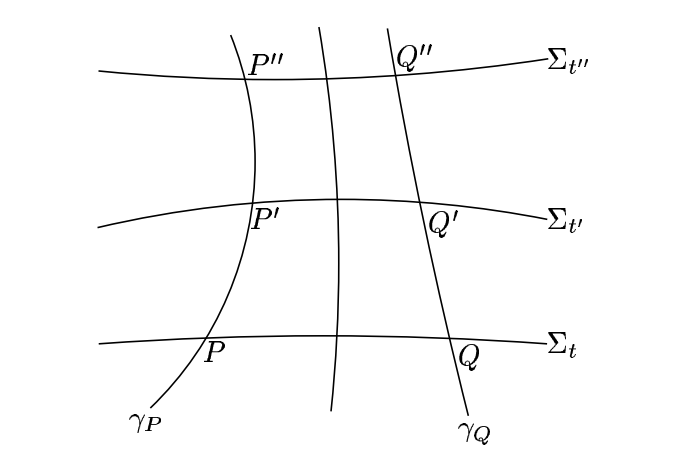
\includegraphics[width=3.5in]{GR/Foliation1.png}
\caption{Foliation of space-time by spacelike hypersurfaces}
\label{fig:side:a}
\end{minipage}%
\begin{minipage}[t]{0.5\linewidth}
\centering
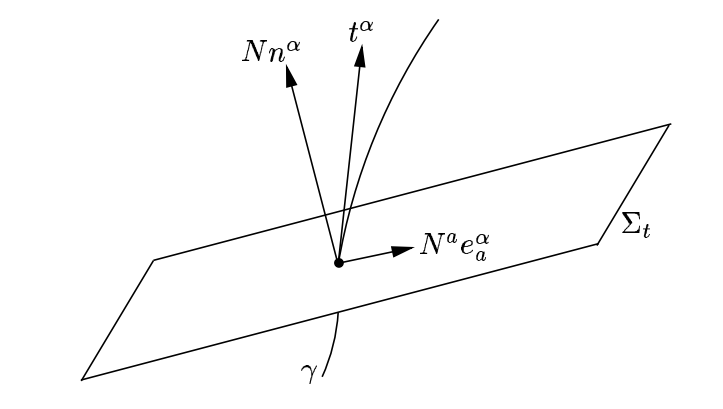
\includegraphics[width=3.5in]{GR/Foliation2.png}
\caption{Decomposition of $t^{\alpha}$ into lapse and shift}
\label{fig:side:b}
\end{minipage}
\end{figure}
\noindent
The space-time is foliated by spacelike hypersurfaces $\Sigma_t$ that is described by scalar function $t(x^{\alpha})$. $t$ is a single valued function and the unit normal to the hypersurfaces $n_{\alpha} \propto \partial_{\alpha} t$ is a future directed timelike vector field.\\
Consider a congruence of curves $\gamma$ intersecting $\Sigma_t$. We use $t$ as a parameter on the curves and the vector $t^{\alpha}$ is tangent to the congruence (so, $t^{\alpha} \partial_{\alpha}t = 1$).Install coordinates $y^a$ on $\Sigma_t$ and impose $y^a(P'') = y^a(P') = y^a(P)$, so $y^a$ is held constant on each member of the congruence. This construction defines a coordinate system $(t,y^a)$ in $\mathcal{V}$.\\
\subsubsection{base vector}
\[t^{\alpha} = \left( \frac{\partial x^{\alpha}}{\partial t}\right)_{y^a}, \ \ \ \ e_a^{\alpha} = \left(\frac{\partial x^{\alpha}}{\partial y^a} \right)_t, \ \ \ \ \mathcal{L}_t e_a^{\alpha} = 0\]
\subsubsection{Normal vector}
\[n_{\alpha} = -N \partial_{\alpha}t, \ \ \ \ n_{\alpha} e_a^{\alpha} = 0\]
\subsubsection{Decomposition of $t^{\alpha}$}
\[t^{\alpha} = N n^{\alpha} + N^a e_a^{\alpha}\]
\subsubsection{Metric}
\begin{eqnarray}
ds^2 &=& g_{\alpha \beta} dx^{\alpha} dx^{\beta} \nonumber \\
&=& g_{\alpha \beta} (t^{\alpha} dt + e_a^{\alpha}dy^a) (t^{\beta} dt + e_b^{\beta}dy^{b}) \nonumber \\
&=& -N^2 dt^2 + h_{ab}(dy^a+N^a dt)(dy^b + N^b dt) \nonumber \\
\sqrt{-g} &=& N \sqrt{h} \nonumber
\end{eqnarray}

\subsection{Field theory}
\[\dot{q} = \frac{\partial q}{\partial t}, \ \ \ \ p=\frac{\partial}{\partial \dot{q}}(\sqrt{-g} \mathcal{L})\]
\[\mathcal{H}(p,q,q_a) = p\dot{q} - \sqrt{-g} \mathcal{L}\]
\[H = \int_{\Sigma_t} \mathcal{H}(p,q,q_{,a})d^3y\]
\[S = \int_{t_1}^{t_2} dt \int_{\Sigma_t} (p \dot{q} - \mathcal{H} ) d^3 y\]
\[\delta S = 0 \Rightarrow \dot{p} = -\frac{\partial \mathcal{H}}{\partial q} + \left(\frac{\partial \mathcal{H}}{\partial q_{,a}}\right)_{,a}, \ \ \ \ \dot{q} = \frac{\partial \mathcal{H}}{\partial p}\]
\begin{example}
For electromagnetic field in 3+1 decomposition form, we define the electrical field as $E_a = F_{\alpha \beta} n^{\beta} e_a^{\alpha}$, the magnetic field as $\epsilon_{abc} B^c = F_{\alpha \beta} e_a^{\alpha} e_b^{\beta}$. In this definition, the equation of motion of particles in electromagnetic field can be written as
\[m A_a = \gamma e (E_a + \epsilon_{abc} v^b B^c)\]
Here, $A_a = u_{\alpha;\beta} u^{\beta} e_a^{\alpha}$, $\gamma = \frac{1}{\sqrt{1-v^2}}$. So, the three force
\[\bm {f}=\frac{d\bm {p}}{dt} = e(\bm {E} + \bm {v} \times \bm {B})\]
If we adopt the coordinates $(t,y^a)$, it is easy to verify that
\[E^a = N F^{0a}, \ \ \ \ B^a = \frac{1}{2} \epsilon^{abc} F_{bc}\]
We further define
\[\mathcal{E}^a = \sqrt{h} E^a, \ \ \ \ \mathcal{B}^a = \sqrt{h} B^a, \ \ \ \ \phi = - A_0, \ \ \ \ \rho_{e} = -j^{\alpha} n_{\alpha} = N j^0\]
If we notice that
\[F_{0a} = -h_{ab}N^2F^{0b} - F_{ab}N^b, \ \ \ \ \tilde{\epsilon}_{abc} \tilde{\epsilon}_{ijk} h^{ai} h^{bj} = \frac{2h_{ck}}{h}\]
It is easy to verify that
\[ \sqrt{-g} \mathcal{L} = - \mathcal{E}^a \dot{A_a} + \phi \mathcal{E}^a_{,a} - \frac{1}{2} N h^{-\frac{1}{2}} h_{ab} (\mathcal{E}^a \mathcal{E}^b + \mathcal{B}^a \mathcal{B}^b) + \tilde{\epsilon}_{abc}N^a \mathcal{E}^b \mathcal{B}^c -\sqrt{h} \phi \rho_e + N \sqrt{h} A_a j^a\]
So,$\pi^a = -\mathcal{E}^a$, and we can get the Hamilton density
\[\mathcal{H} = \phi \pi^a_{,a} + \frac{1}{2} N h^{-\frac{1}{2}} h_{ab} (\pi^a \pi^b + \mathcal{B}^a \mathcal{B}^b) + \tilde{\epsilon}_{abc}N^a \pi^b \mathcal{B}^c +\sqrt{h} \phi \rho_e - N \sqrt{h} A_a j^a\]
Then, the Hamilton equation can be written as
\[\dot{A}_a = -\phi_{,a} + N h^{-\frac{1}{2}} h_{ab}\pi^b + \tilde{\epsilon}_{abc}N^a \mathcal{B}^c\]
\[\dot{\pi}^a = - \tilde{\epsilon}^{jab}(Nh^{-\frac{1}{2}}h_{ij}\mathcal{B}^i)_{,b} - \tilde{\epsilon}^{cab}(\tilde{\epsilon}_{ijc}N^i \pi^j)_{,b} + N\sqrt{h}j^a \]
and also the constraint equation $\pi^a_{,a} + \sqrt{h}\rho_e = 0$.
After simplification, the Maxwell equations are
\begin{eqnarray}
\frac{1}{\sqrt{h}}\frac{\partial}{\partial t}(\sqrt{h} \bm{E}) &=& \nabla \times (N \bm{B} - \bm{N} \times \bm{E}) - N \bm{J} \nonumber \\
\frac{1}{\sqrt{h}}\frac{\partial}{\partial t}(\sqrt{h} \bm{B}) &=& -\nabla \times (N \bm{E} + \bm{N} \times \bm{B}) \nonumber \\
\nabla \cdot \bm{E} &=& \rho_e \nonumber \\
\nabla \cdot \bm{B} &=& 0 \nonumber
\end{eqnarray}
\end{example}


\subsection{General relativity}
\[S_G = \frac{1}{16 \pi} \int_{t_1}^{t_2} dt \left\{ \int_{\Sigma_t} \left(\phantom{R}^3R + K^{ab}K_{ab} -K^2 \right) N \sqrt{h} d^3 y + 2\oint_{\Sigma_t}(k-k_0)N \sqrt{\sigma}d^2 \theta \right\} \]
$k_0 =$ extrinsic curvature of $S_t$ embedded in flat space. 

\subsubsection{Gravitational Hamiltonian}
\[\dot{h}_{ab} \equiv \mathcal{L}_t h_{ab} = \mathcal{L}_t (g_{\alpha \beta} e_a^{\alpha} e_b^{\beta}) =  2NK_{ab} + N_{a|b} + N_{b|a})\]
\[K_{ab} = \frac{1}{2N} (\dot{h}_{ab} - N_{a|b} - N_{b|a})\]
\[p^{ab} = \frac{\partial}{\partial \dot{h}_{ab}} (\sqrt{-g} \mathcal{L}_G) = \frac{\sqrt{h}}{16\pi} (K^{ab} - K h^{ab})\]
\[\sqrt{h}K^{ab} = 16\pi (p^{ab} - \frac{1}{2}ph^{ab})\]
\[\mathcal{H}_G = p^{ab}\dot{h}_{ab} - \sqrt{-g} \mathcal{L}_G\]
\begin{eqnarray}
16\pi H_G &=& \int_{\Sigma_t} \left[ N(K^{ab}K_{ab} - K^2 - \phantom{R}^3R) - 2N_a(K^{ab} - Kh^{ab})_{|b} \right] \sqrt{h} d^3 y 
\nonumber \\
&\phantom{=}& -2\oint_{S_t} \left[ N(k-k_0) - N_a(K^{ab}-Kh^{ab})r_b \right] \sqrt{\sigma} d^2 \theta \nonumber
\end{eqnarray}

\subsubsection{Variation of gravitational Hamiltonian}
\[\delta N = \delta N^a = \delta h_{ab} = 0 \mbox{ on } S_t\]
\[\delta H_G = \int_{\Sigma_t} (\mathcal{P}^{ab} \delta h_{ab} + \mathcal{H}_{ab} \delta p^{ab} - \mathcal{C}\delta N - 2\mathcal{C}_a \delta N^a) d^3 y\]
\begin{eqnarray}
(16\pi)\mathcal{P}^{ab} &=&  N\sqrt{h}G^{ab} - \sqrt{h}(N^{|ab} - h^{ab} N^{|c}_{\phantom{|c}c}) \nonumber \\
&\phantom{=}& +(16\pi)[2p^{c(a}N^{b)}_{\phantom{b)}|c} - \sqrt{h}(\frac{1}{\sqrt{h}}p^{ab}N^c)_{|c}] \nonumber \\
&\phantom{=}& + (16\pi)^2 [\frac{2N}{\sqrt{h}} (p^a_c p^{bc} - \frac{1}{2} p p^{ab}) - \frac{N}{2\sqrt{h}}(p^{cd}p_{cd} - \frac{1}{2} p^2)h^{ab}] \nonumber \\
\mathcal{H}_{ab} &=& (16\pi) \frac{2N}{\sqrt{h}} (p_{ab} - \frac{1}{2}p h_{ab}) + 2N_{(a|b)} \nonumber \\
\mathcal{C} &=& \frac{\sqrt{h}}{16\pi} (\phantom{R}^3R + K^2 - K^{ab}K_{ab}) \nonumber \\
\mathcal{C}^a &=& \frac{\sqrt{h}}{16\pi} (K_a^{\phantom{a}b} - K \delta_a^{\phantom{a}b})_{|b} \nonumber 
\end{eqnarray}

\subsubsection{Variation of electromagnetic Hamiltonian}
\[\delta H_E = \int_{\Sigma_t}(-\frac{1}{2}N\sqrt{h}\mathcal{I}^{ab} \delta h_{ab} + \sqrt{h} \rho \delta N - \sqrt{h} s_a \delta N^a)\]
\begin{eqnarray}
\mathcal{I}^{ab} &=& \frac{1}{2}(E^c E_c + B^c B_c)h^{ab} - E^a E^b - B^a B^b \nonumber \\
\rho &=& \frac{1}{2}(E^c E_c + B^c B_c) \nonumber \\
s_a &=& \epsilon_{abc} E^b B^c \nonumber
\end{eqnarray}

\subsubsection{Hamilton's equations}
\[\dot{h}_{ab} = \mathcal{H}_{ab}, \ \ \ \ \dot{p}^{ab} = -\mathcal{P}^{ab}+\frac{1}{2}N\sqrt{h}\mathcal{I}^{ab}\]
\[\phantom{R}^3R + K^2 - K^{ab}K_{ab} = 16 \pi \rho\]
\[(K_a^{\phantom{a}b} - K \delta_a^{\phantom{a}b})_{|b} = -8\pi s_a\]


